As a first qualitative test to the code, we consider the decay of a wide range of nuclei, from $(Z,N)=(10,10)$ to $(90,130)$.
A list of all eligible nuclei was generated by \prgname{nuclist}, for 4 different exciation energies, $E*=\unit[5, 10, 15, 20]{MeV}$, and $J=0$ was generated using \prgname{Nuclist}. The most likely decay channel of these nuclei were then calculated with \prgname{spectra}.

The results, which were run though an \prgname{Octave} script to plot each nuclei on a chart, is presented in \autoref{fig:chart1} and \autoref{fig:chart2}. In the first picture, we see how the nuclei close to the line of $\beta$-stability preferentially decay by emitting a gamma at $E^*=\unit[5]{MeV}$, but already at $E^*=\unit[10]{MeV}$, most nuclei are \emph{particle unstable}. Proton separation energies for stable nuclei are in the range of $\unit[7-9]{MeV}$\cite{audi:1995}, so these results should be reasonable.
We also see a distinct odd-even effects: nuclei with an even number of a nucleon tend to have higher separation energies, due to pairing. Finally, we note that neutron evaporation is by far more common across the chart, which is to be expected, since protons have to tunnel through the Coulomb barrier. %The line $Z=N$, rather than the line of $\beta$-stability, seem to be a decent indicator of where \codename{} predicts the line between neutron and proton emission to be.
Note however that our Fermi-gas level density will not be valid for low energies, where the discreteness of the levels should be taken into account -- these results should be viewed more like a benchmark of the code, than physical predictions.

At yet higher energies, a few potential oddities appear. According to \codename{}, relatively neutron rich nuclei decay by emitting a proton -- neutron rich meaning below the region of ``proton instability'', and in one case even below the line of $\beta$-stability!
It could perhaps be that once the energy is high enough for protons to readily tunnel through the Coulomb barrier, a high level density in the daughter nucleus makes the program favor proton decay. 
This kind of reasoning could also be applied to alpha particles, which have a higher Coulomb barrier, but may be allowed to dominate at sufficiently high energies if the level density of the daughter is favorable. However, we see a few nuclei, $(Z,N)=(17,15); (32,33); (33,34)$ that decay by proton evaporation at $E^*=\unit[10]{MeV}$, then by $\alpha$ at $E^*=\unit[15]{MeV}$ and by proton at $E^*=\unit[20]{MeV}$, which could indicate that there is no simple energy threshold above which more \emph{density favored} decay start to dominate. However, $\alpha$ and protons have vastly different centrifugal barriers, which perhaps may explain the more complicated shifts in prefered decay modes.

\afterpage{
\begin{figure}
\thisfloatpagestyle{empty}
\begin{center}
\begin{tabular}{c}
\subfloat[$E^{*}=5\,\mathrm{MeV}$]{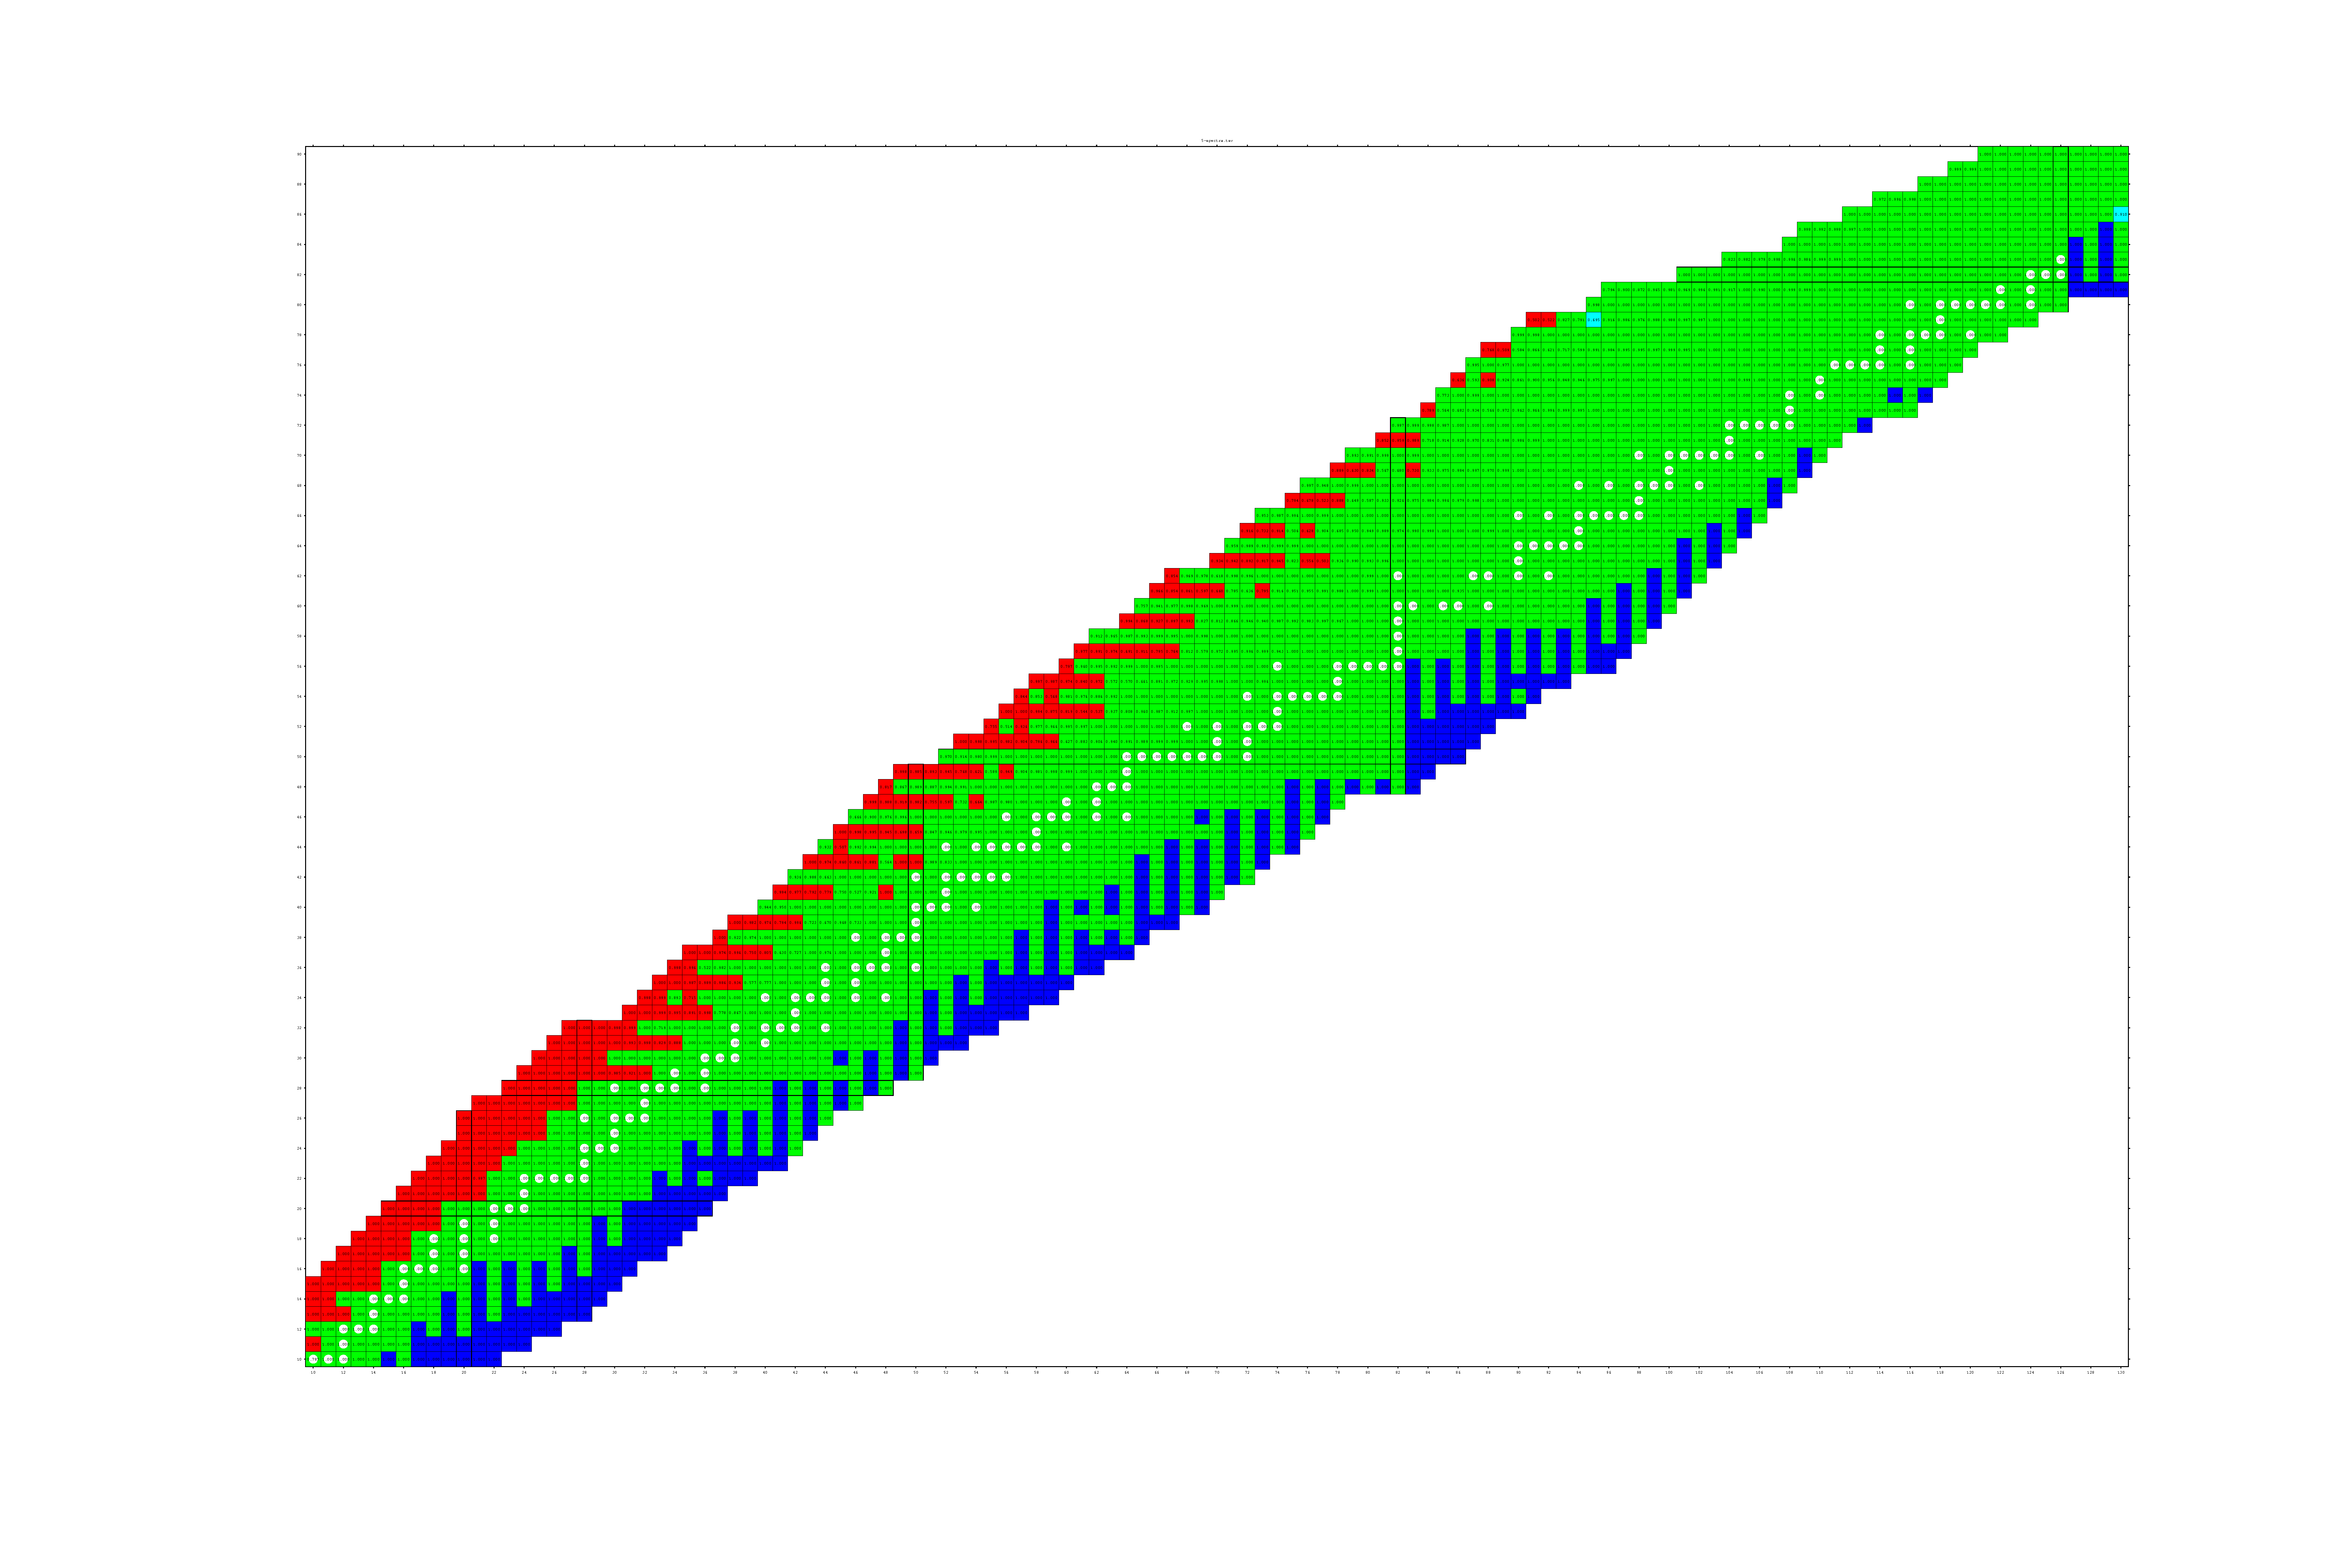
\includegraphics[width=\textwidth]{figures/spectra/5-spectra.pdf}\label{sfig:chart1:5}}
\\
\subfloat[$E^{*}=10\,\mathrm{MeV}$]{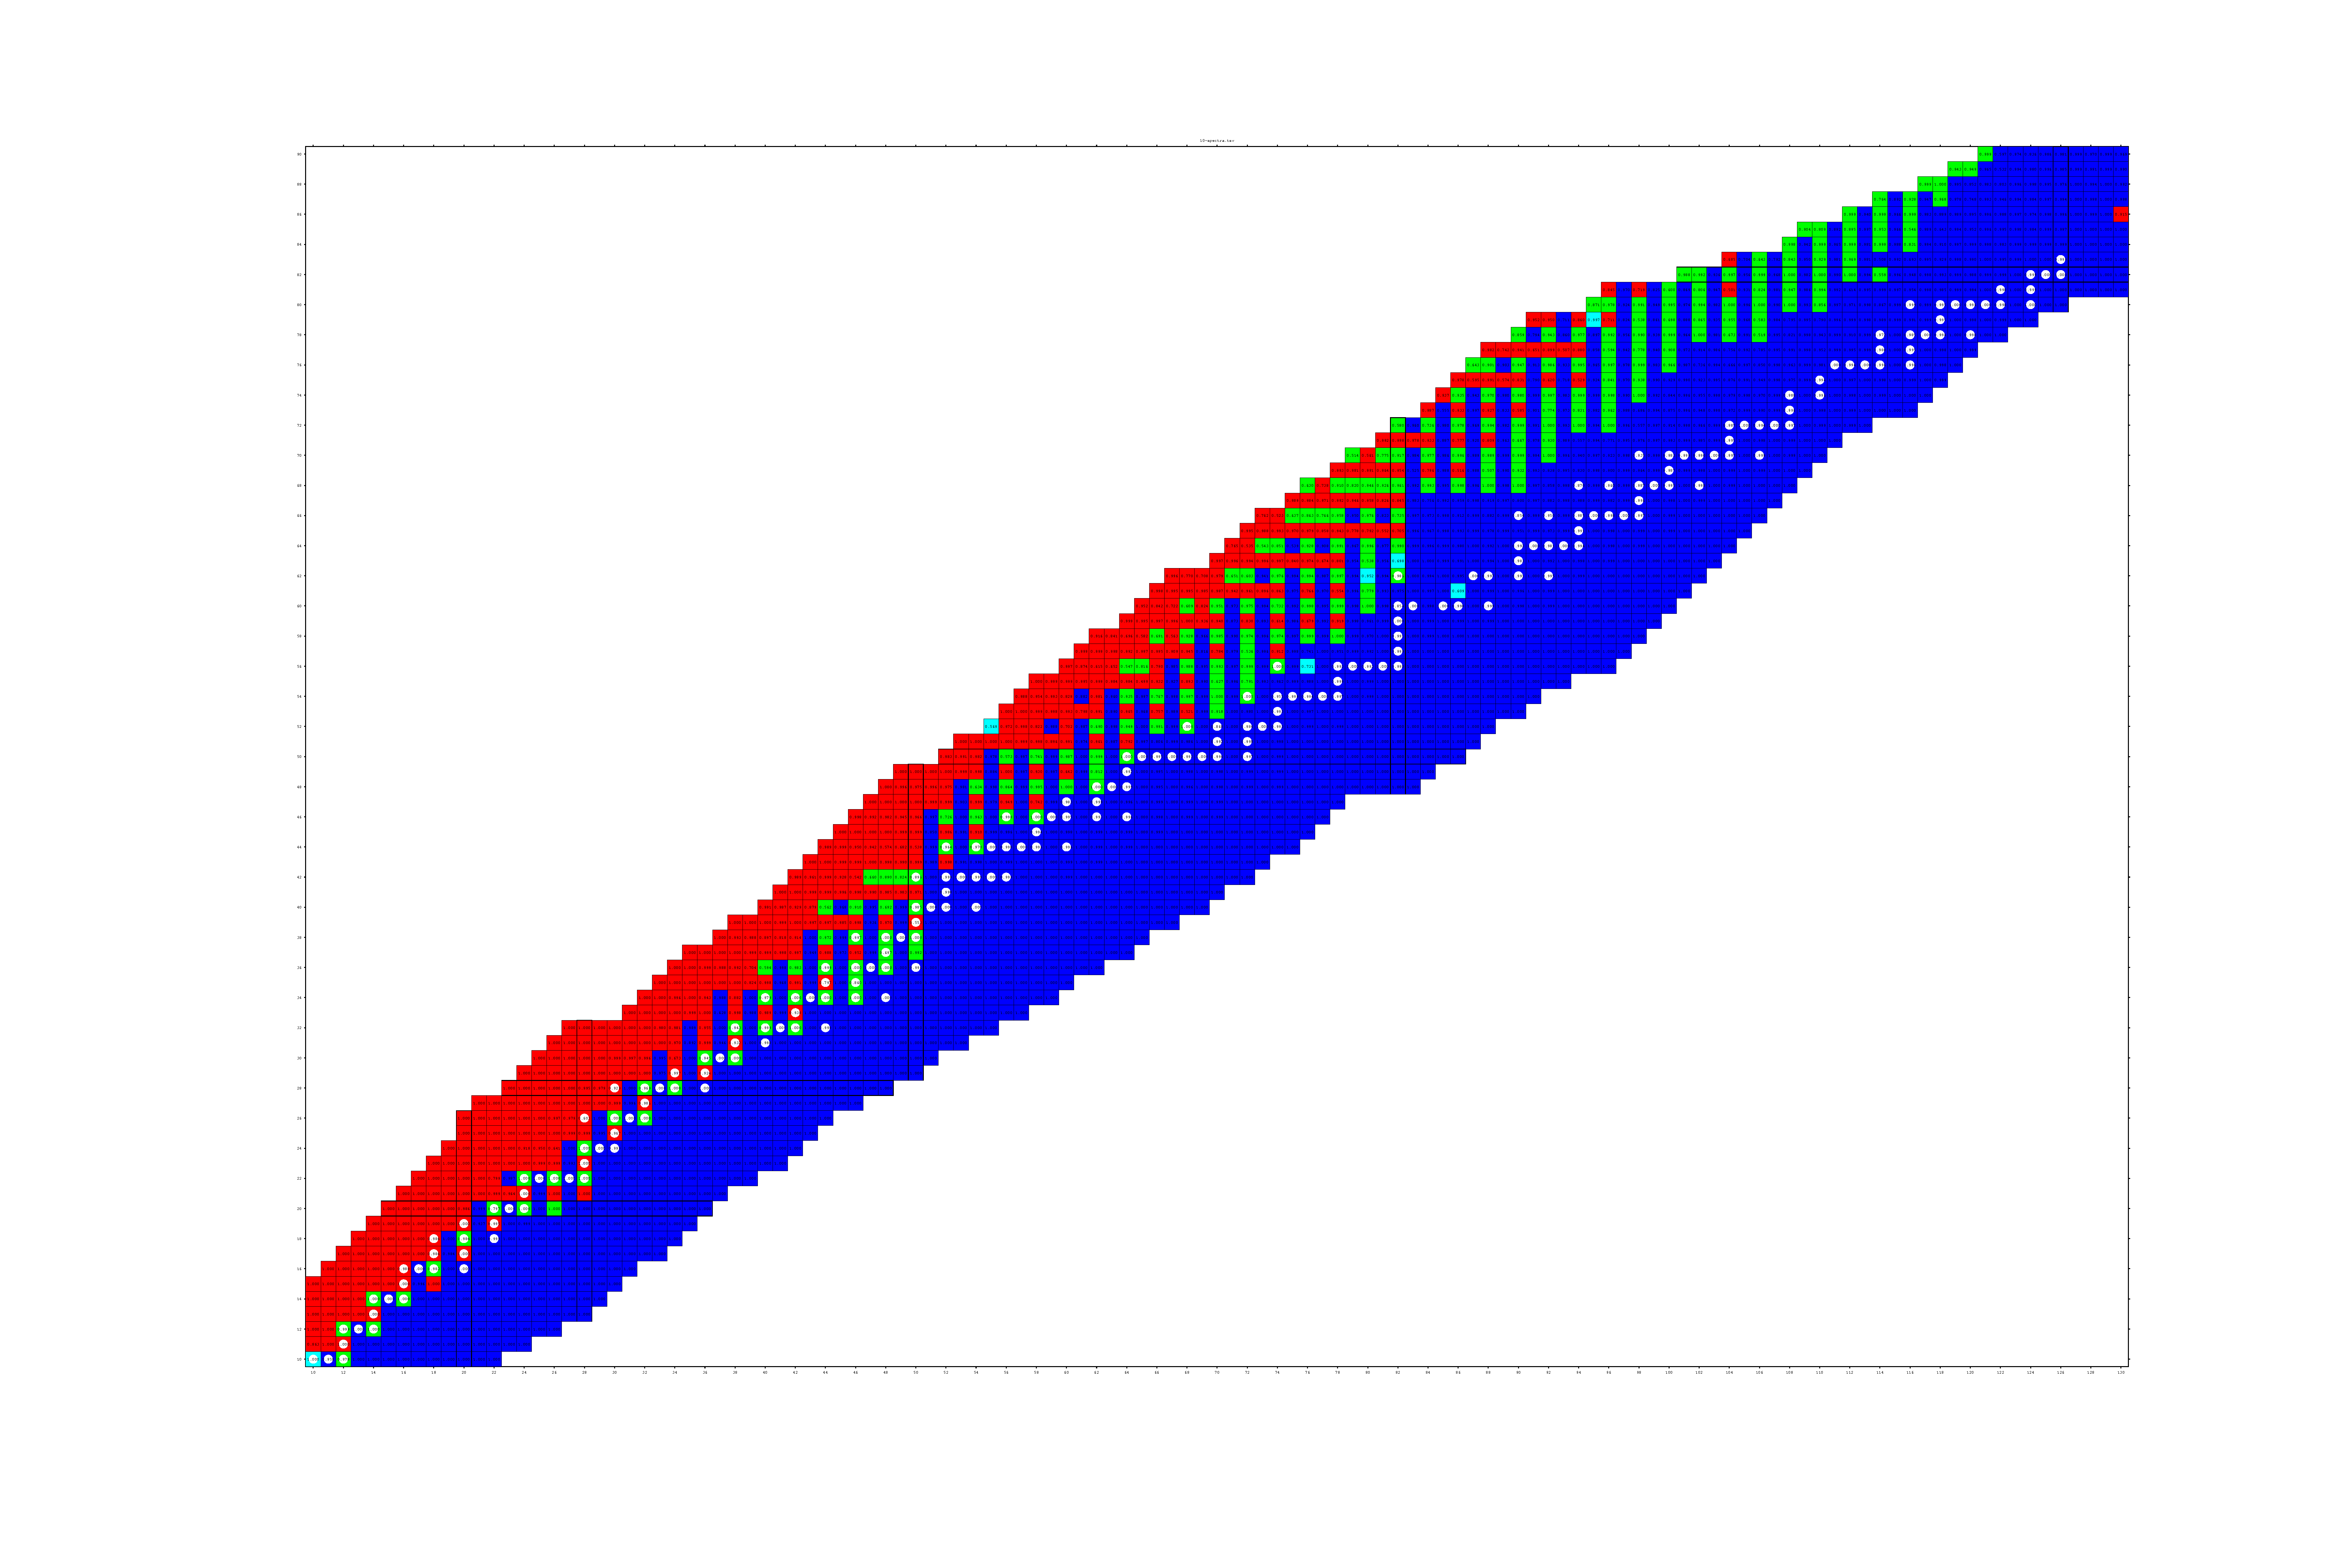
\includegraphics[width=\textwidth]{figures/spectra/10-spectra.pdf}\label{sfig:chart1:10}}
\end{tabular}
\caption{\label{fig:chart1} The prefered decay mode of a wide range of nuclei according to \codename{}, for various excitation energies and $J=0$. The dominant decay mode is indicated as follows: blue=neutron, red=proton, green=gamma, cyan=alpha. Nuclei that are beta-stable in their ground-state are marked with a white dot.}
\end{center}
\end{figure}
\begin{figure}
\thisfloatpagestyle{empty}
\begin{center}
\begin{tabular}{c}
\subfloat[$E^{*}=15\,\mathrm{MeV}$]{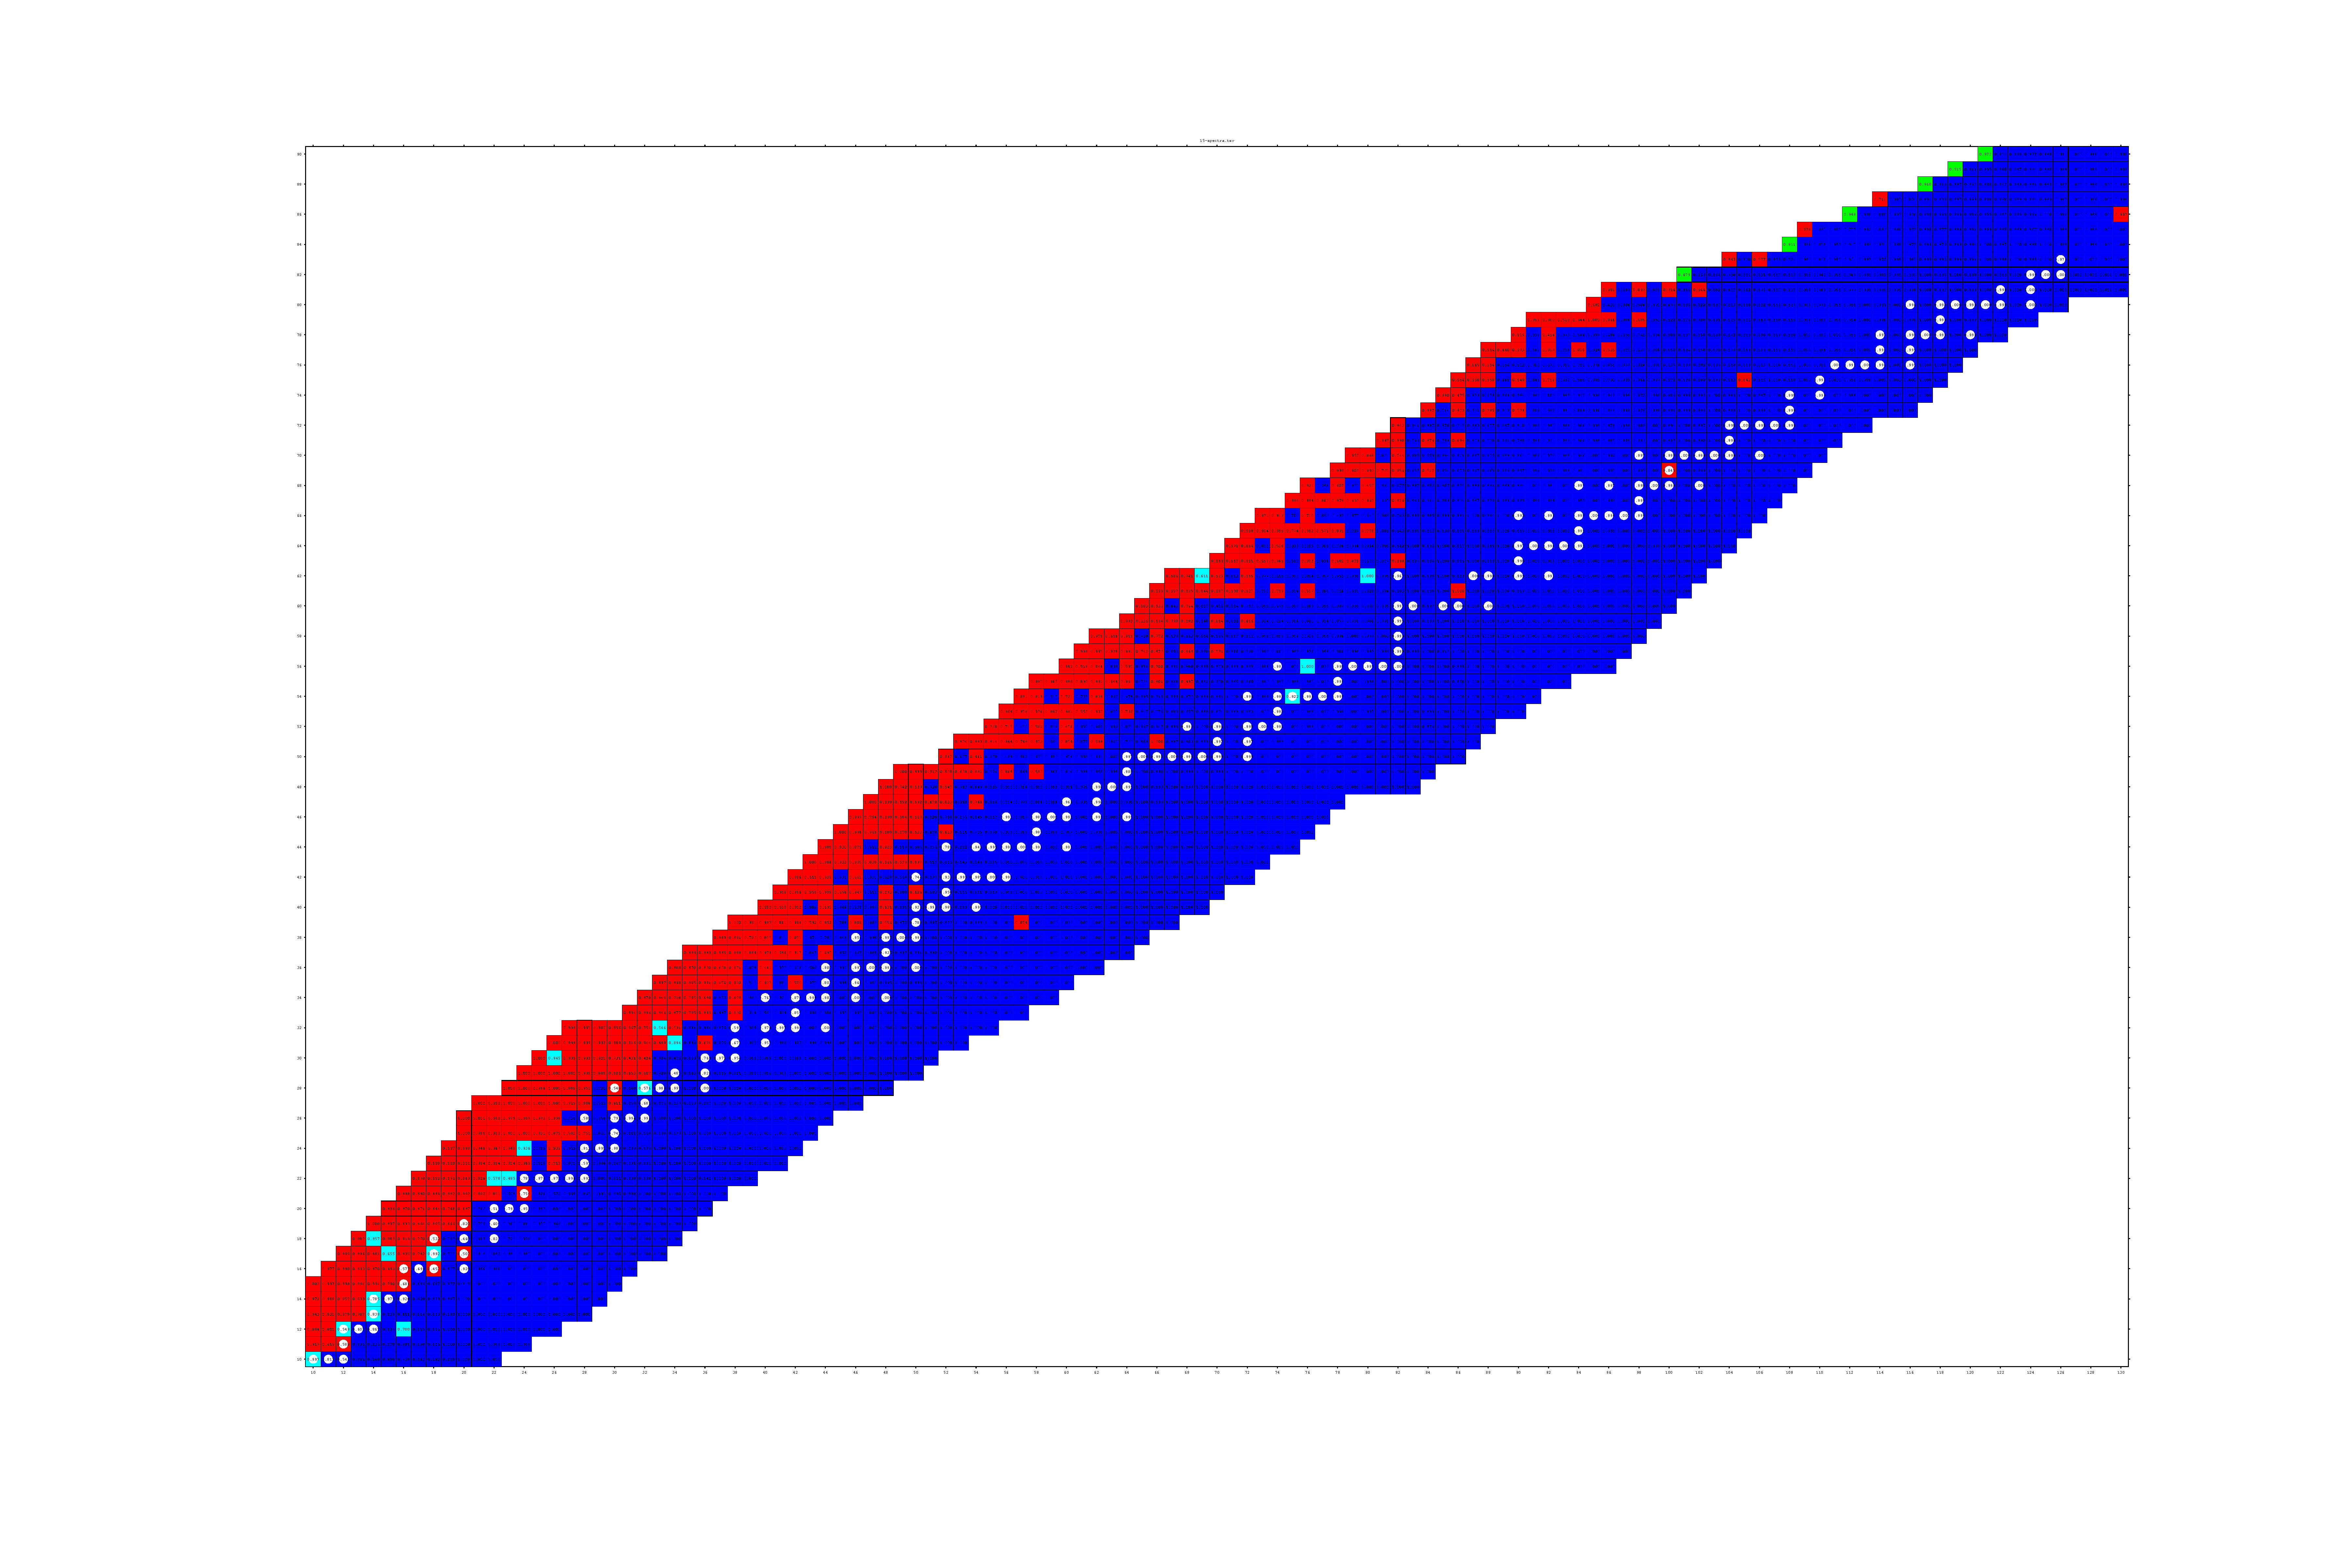
\includegraphics[width=\textwidth]{figures/spectra/15-spectra.pdf}\label{sfig:chart2:15}}
\\
\subfloat[$E^{*}=20\,\mathrm{MeV}$]{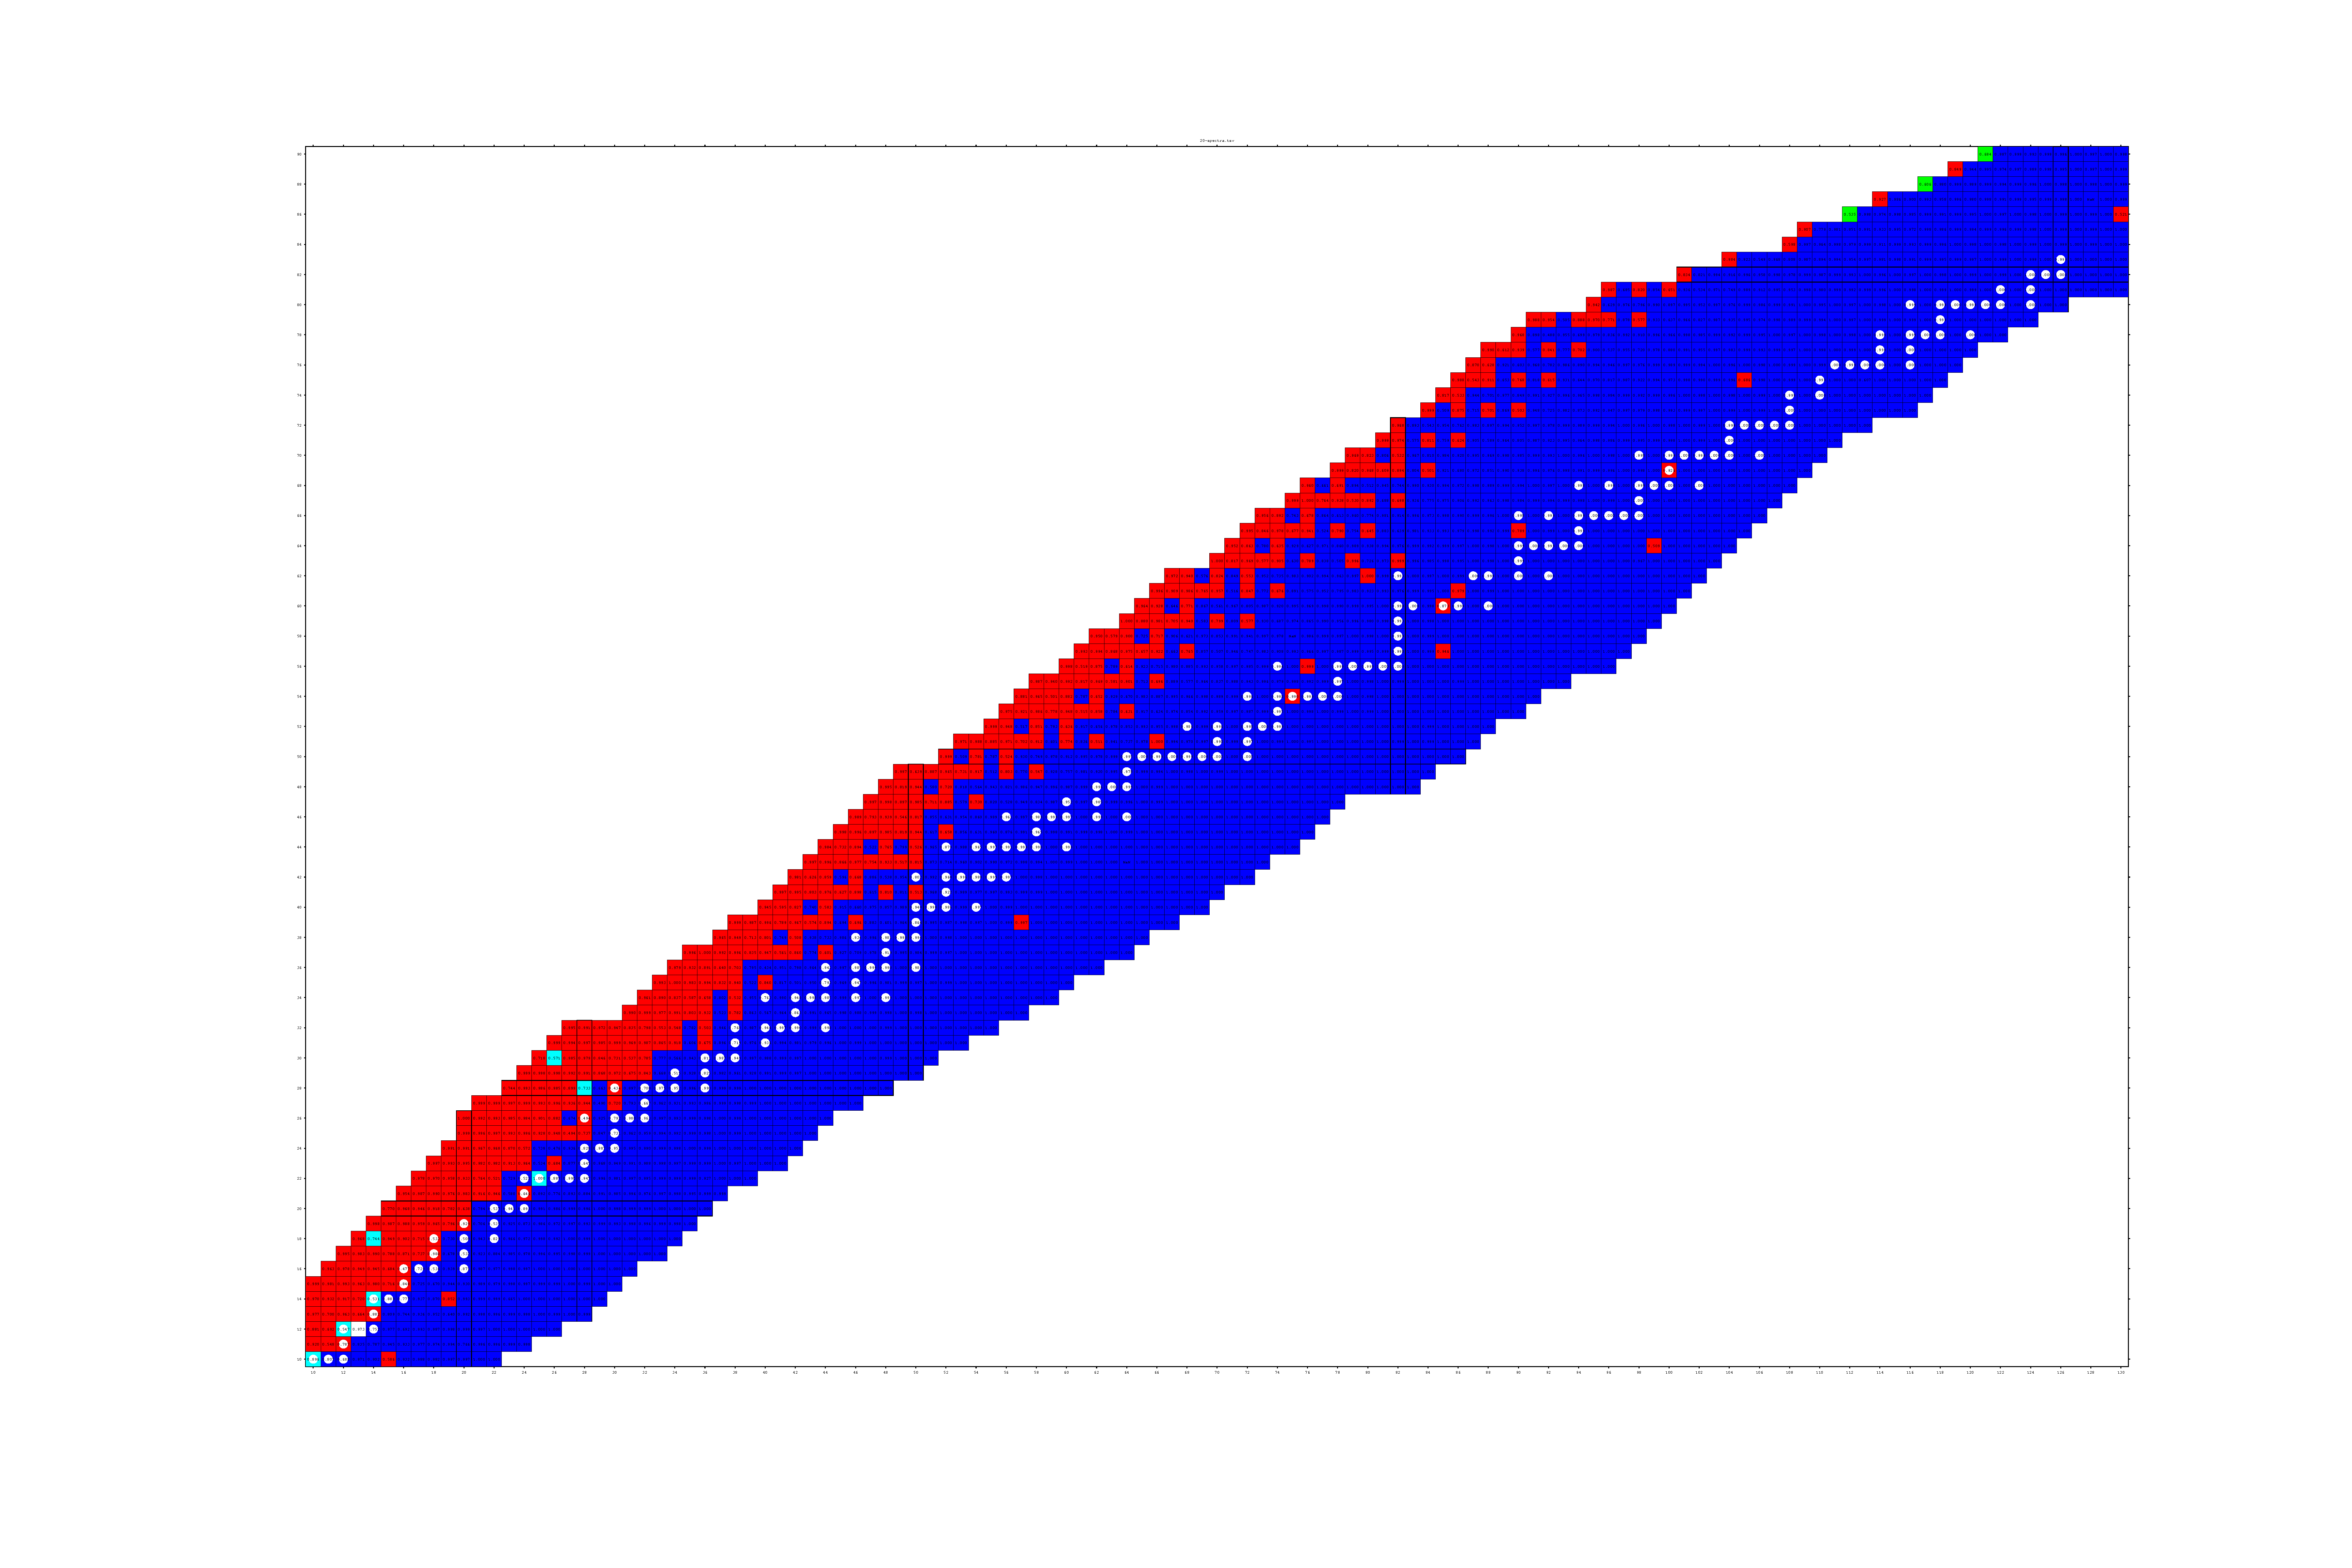
\includegraphics[width=\textwidth]{figures/spectra/20-spectra.pdf}\label{sfig:chart2:20}}
\end{tabular}
\caption{\label{fig:chart2} The prefered decay mode of a wide range of nuclei according to \codename{}, for various excitation energies and $J=0$. The dominant decay mode is indicated as follows: blue=neutron, red=proton, green=gamma, cyan=alpha. Nuclei that are beta-stable in their ground-state are marked with a white dot.}
\end{center}
\end{figure}
}
\clearpage

These results where compared with the output of another nuclear reaction code, \prgname{Talys}\cite{talys:2015}. Specifically, \prgname{Talys-1.73} was used, since it adds a keyword to make \prgname{Talys} print the emission spectra from a specific excited level\footnote{Thanks to Arjan Koning for implementing this!}. 
The results of the \prgname{Talys} simulations can be seen in \autoref{fig:chart-talys}, for $E^*=\unit[20]{MeV}$. This energy was choosen since \prgname{Talys} uses discrete levels for lower excitation energies, and is thus often unable to populate nuclei close to specific energies, such as $E^*\approx\unit[5]{MeV}$.
No restriction on the spin of the levels were imposed, and in the cases where two levels were suitably close to $E^*\approx\unit[20]{MeV}$, the highest level was chosen.
Even then, \prgname{Talys} was unable to populate an $E^*\approx\unit[20]{MeV}$ level for some nuclei (white in \autoref{fig:chart-talys}). In at least one case, $~^{74}\mathrm{Rb}$, this is due to the fact that \prgname{Talys}, by default, uses discrete levels even at $E^*=\unit[20]{MeV}$\footnote{In \prgname{Talys} default files, $~^{74}\mathrm{Rb}$ has very few levels -- not even the 100 levels the manual states that every nuclei should have. These levels go to much higher energies compared to other nuclei, and given how sparse they are, it seems very likely that this is a bug.}. 
In other cases, I believe this is due to how \prgname{Talys} discretizes the continuous energy, since I could populate levels close to \unit[20]{MeV} for other problematic nuclei by changing the energy of the highest discrete level.

We see that the spectra are in qualitative agreement, and that the oddities of the \codename{} output is not present in the \prgname{Talys} results, which one the whole has a less jagged boundary between the region of proton and neutron instability.
\begin{figure}
\begin{center}
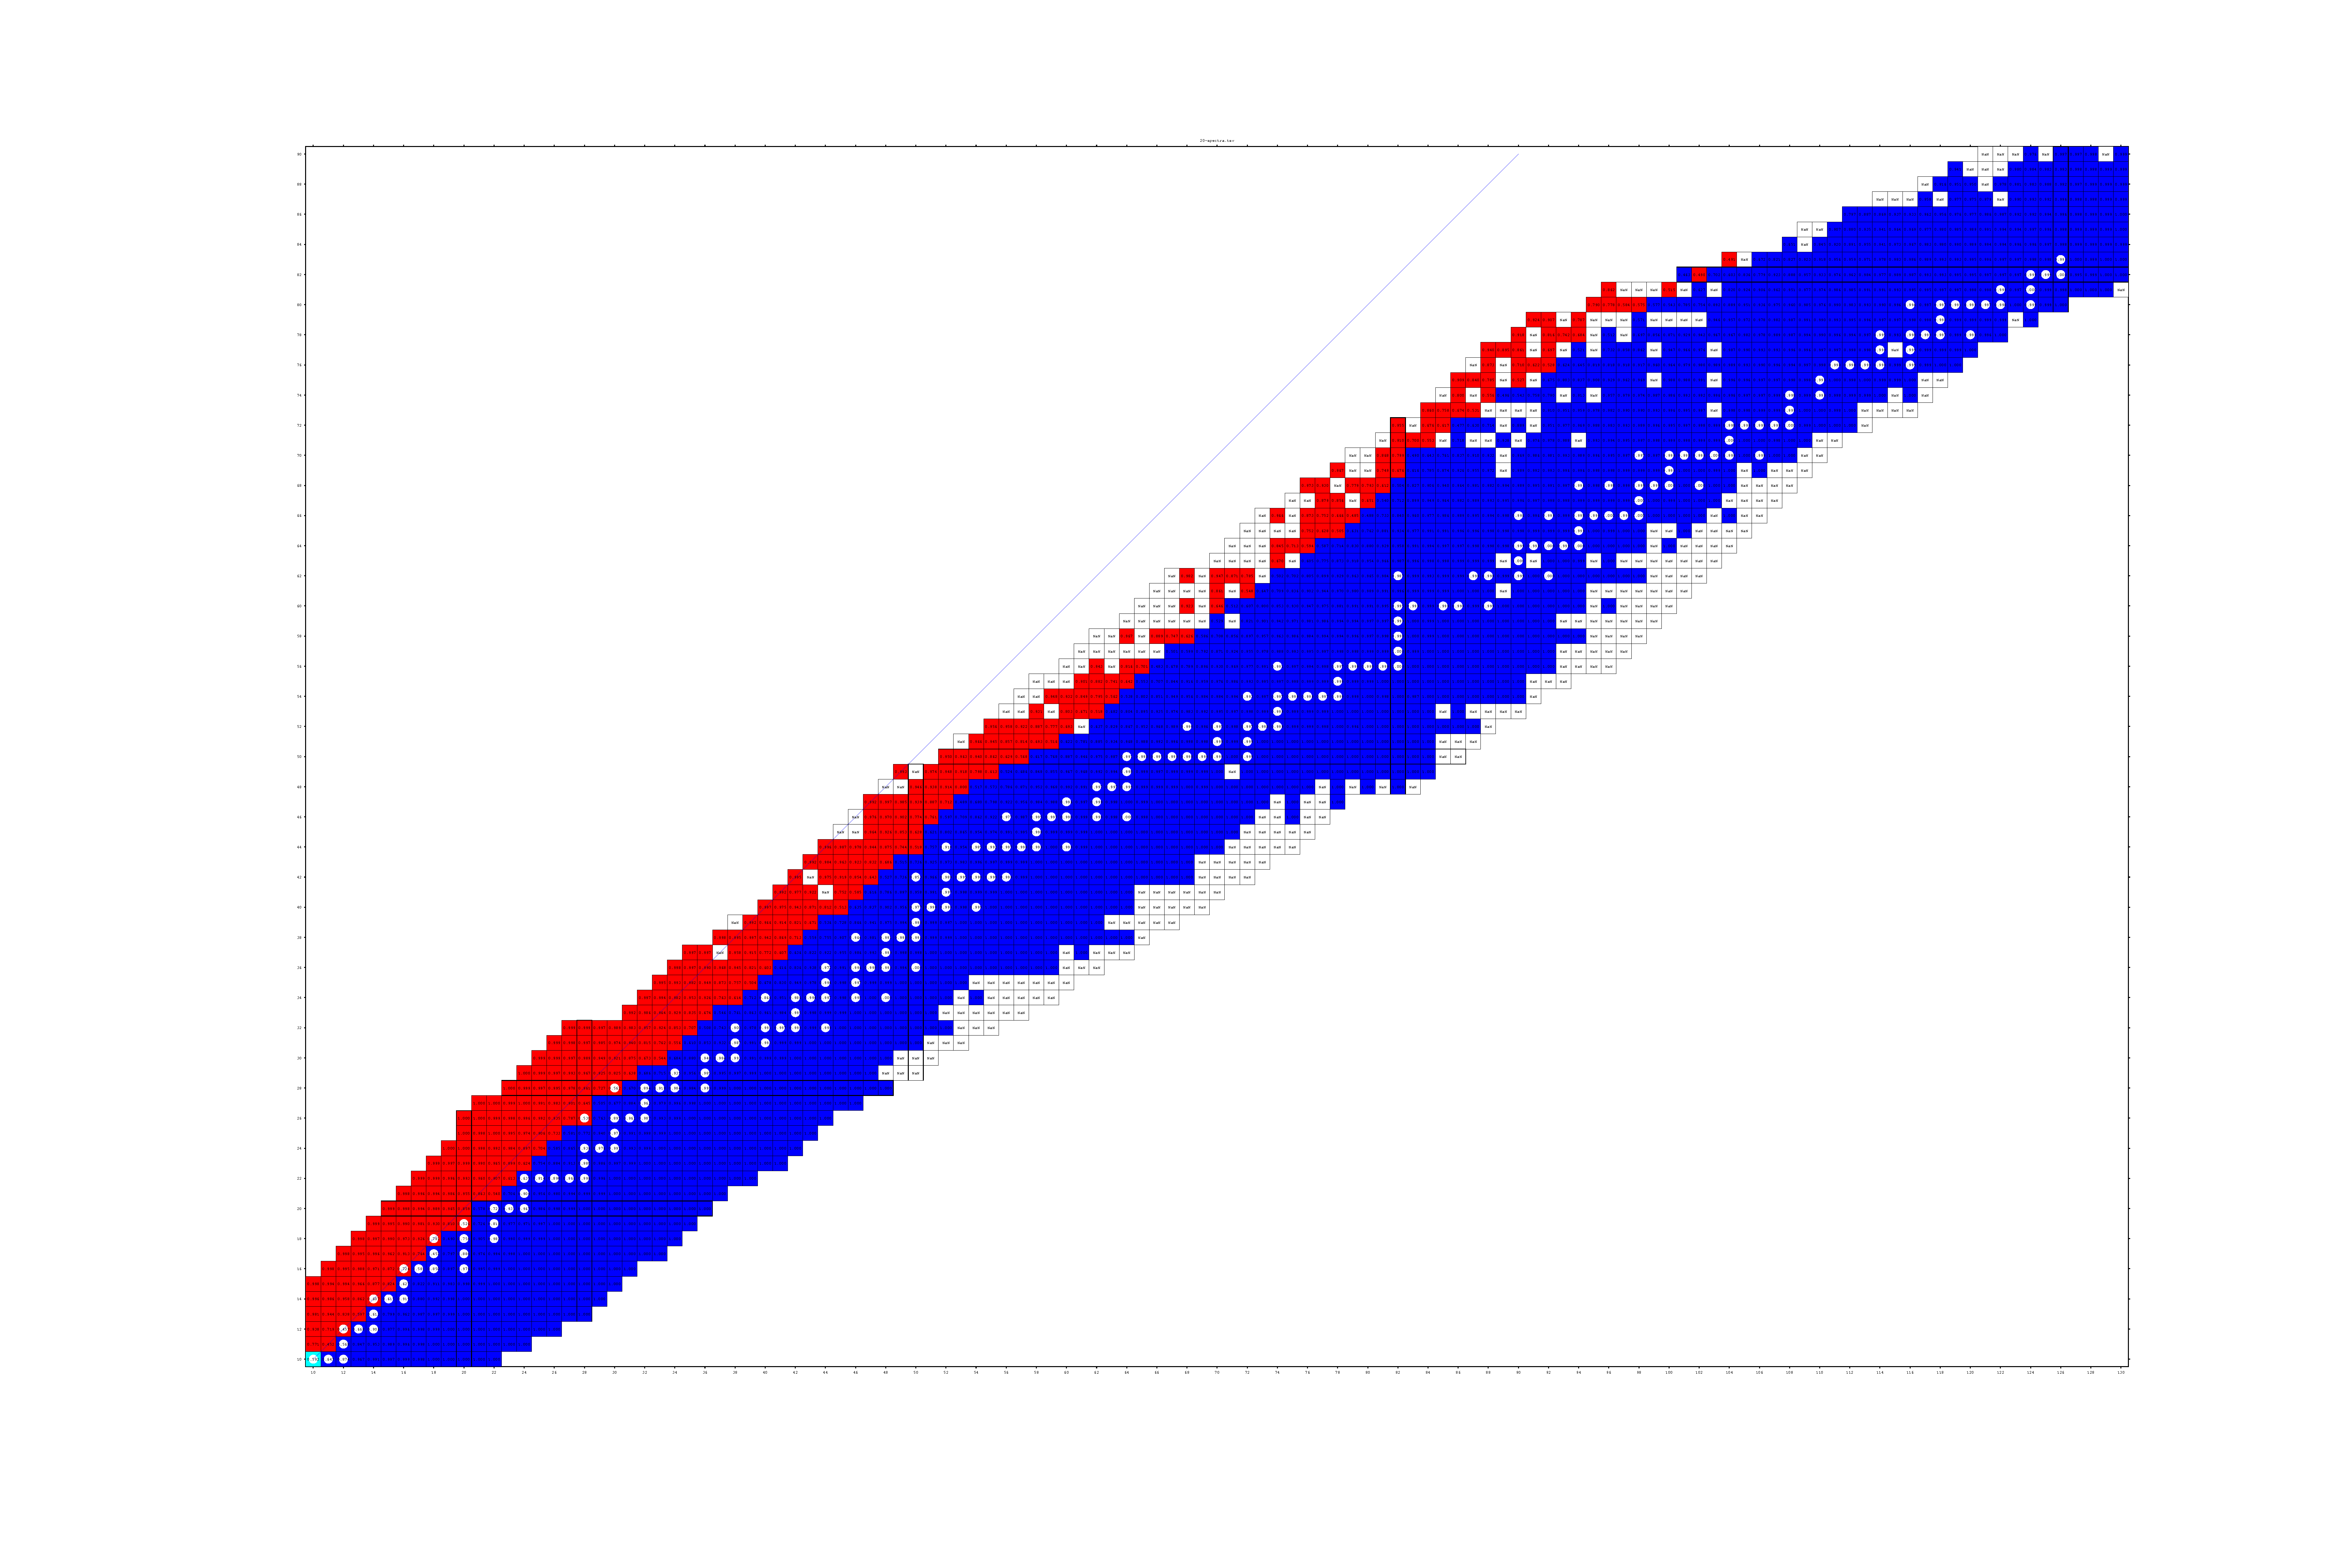
\includegraphics[width=\textwidth]{figures/spectra/talys-20-spectra.pdf}
\caption{\label{fig:chart-talys} The prefered decay mode of various nuclei according to \prgname{Talys}, for the excitation energy $E^*=\unit[20]{MeV}$. The dominant decay mode is indicated as follows: blue=neutron, red=proton, green=gamma, cyan=alpha. Nuclei that are beta-stable in their ground-state are marked with a white dot. Nuclei which had no suitable level near $E^*=\unit[20]{MeV}$ are displayed in white.}
\end{center}
\end{figure}

\subsection{A more detailed spectra of the $A=28$ isobar.}
In order to investigate how the region of proton and neutron instability evolves with higher excitation energies, we look at the particle spectra of the $A=28$ isobar. This isobar was chosen since it displays some of the anomalous behavior discussed above, and since we eventually want to focus on lighter nuclei when we later apply the code. The behaviour for lower energies is illustrated in \autoref{fig:bars1}. $~^{28}F$ is neutron unbound, while the other nuclei start to decay dominantly by neutron and proton emission almost as soon as they pass over the separation energies, which is presented in \autoref{tab:sep}. At even higher energies, as presented in \autoref{fig:bars2}, alpha evaporation starts to become energetically possible, and also -- apparently -- tritium evaporation, although that has a low probability of occuring. At yet higher energies, \autoref{fig:bars3}, the probabilty for alpha decay starts to decrease again -- possibly due to evaporation of partilces in higher $l$-states becoming possible for the lighter particles. For comparison, the output spectra from \prgname{Talys} at $E^*=\unit[20]{MeV}$ is presented in \autoref{fig:barst}. Notably, the $\alpha$-branching ratio is significantly lower for $~^{28}\mathrm{Si}$.

\begin{figure}
\begin{center}
\begin{tabular}{cc}
\subfloat[$E^{*}=1\,\mathrm{MeV}$]{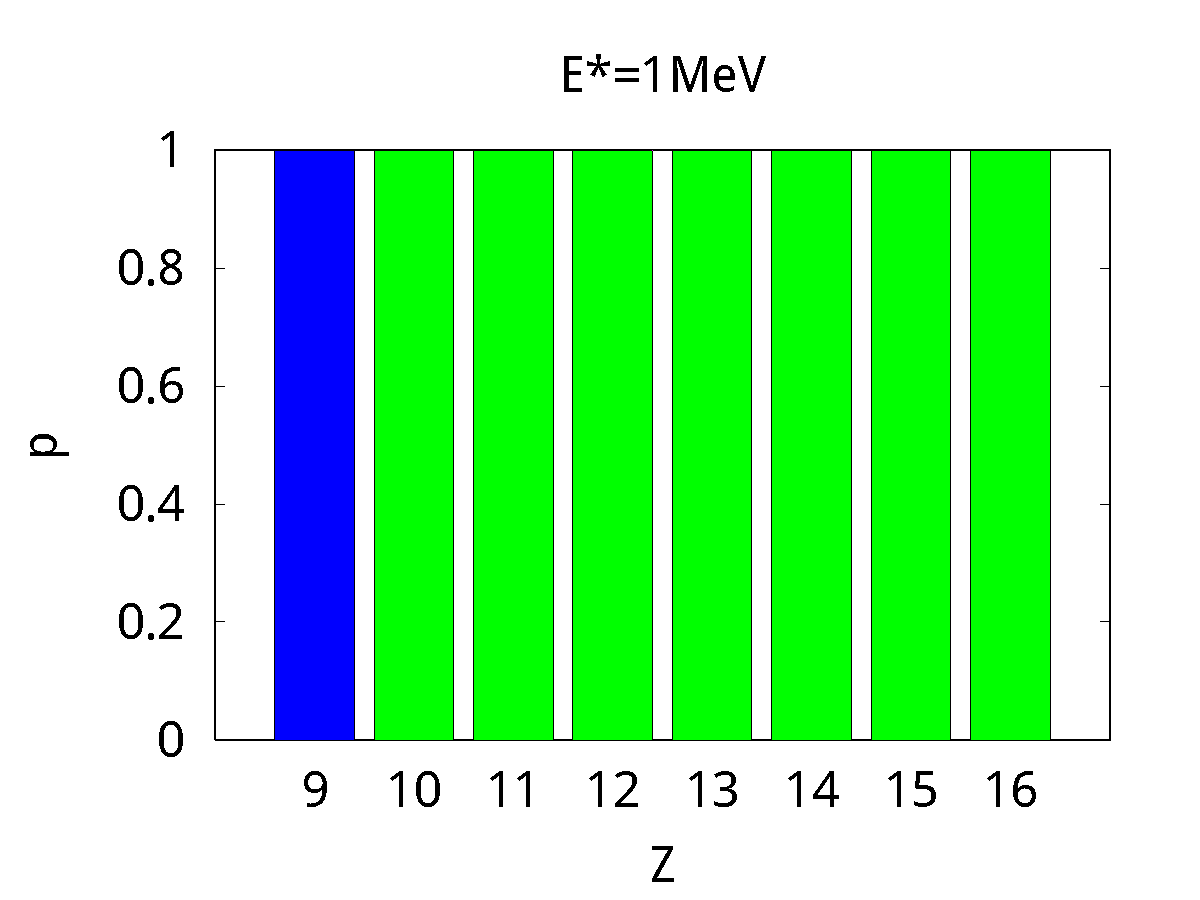
\includegraphics[width=\bredd\textwidth]{figures/bars/1-spectra.pdf}\label{sfig:bars1:1}}
&
\subfloat[$E^{*}=3\,\mathrm{MeV}$]{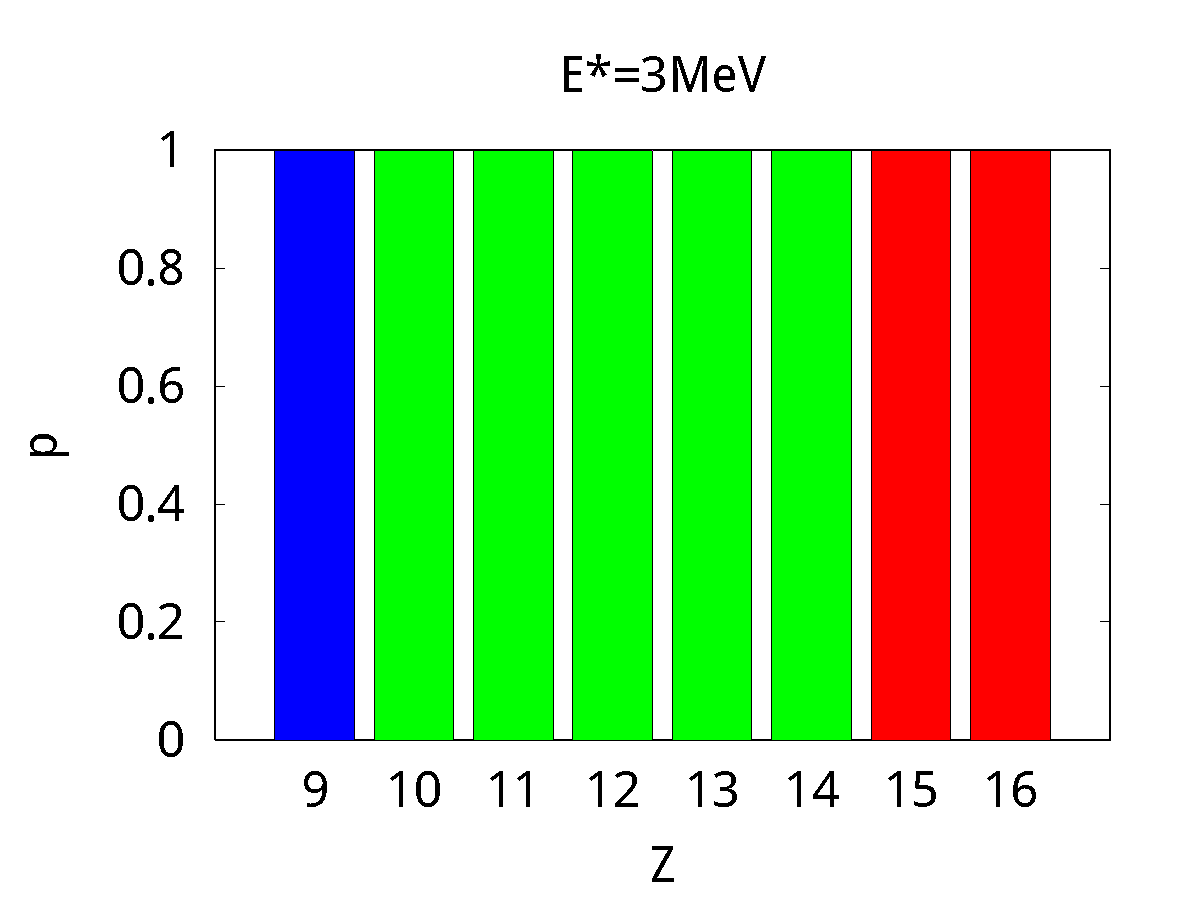
\includegraphics[width=\bredd\textwidth]{figures/bars/3-spectra.pdf}\label{sfig:bars1:3}}
\\
\subfloat[$E^{*}=5\,\mathrm{MeV}$]{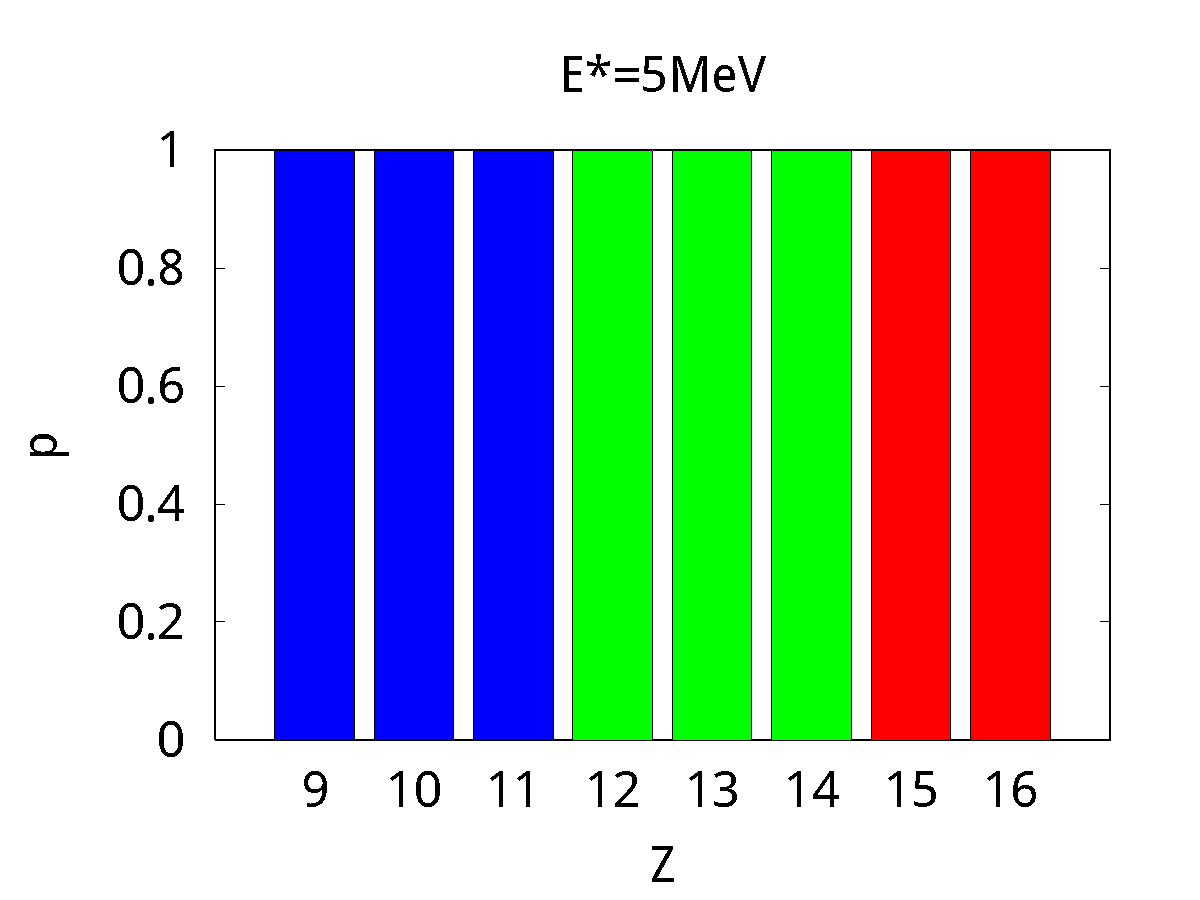
\includegraphics[width=\bredd\textwidth]{figures/bars/5-spectra.pdf}\label{sfig:bars1:5}}
&
\subfloat[$E^{*}=10\,\mathrm{MeV}$]{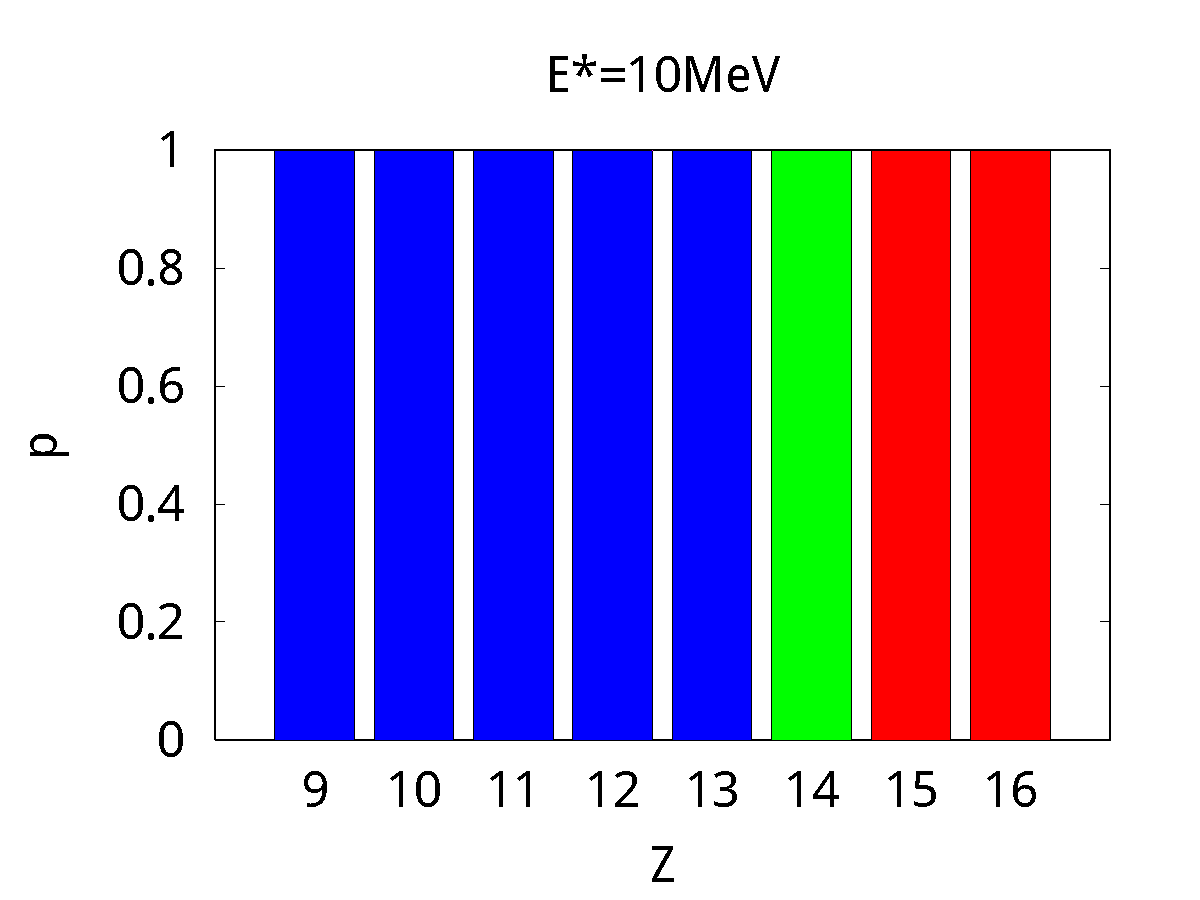
\includegraphics[width=\bredd\textwidth]{figures/bars/10-spectra.pdf}\label{sfig:bars1:10}}
\end{tabular}
\caption{\label{fig:bars1} The branching ratios for various decay modes at various energies for nuclei in the $A=28$, according to \codename{}. The spin is $J=0$ in all cases. The energies have been chosen to display changes in the spectrum. The colors signify the different decay modes: blue=neutron, red=proton, green=gamma.}
\end{center}
\end{figure}

\begin{table}
\begin{center}
\begin{tabular}{l|lll}
Nucleus & $S_p$ & $S_n$ & $S_\alpha$ (MeV)\\\hline\hline
$~^{28}\mathrm{F}$ & 19.0 & -0.228 & 16.7 \\\hline
$~^{28}\mathrm{Ne}$ & 21.0 & 3.90 & 10.3 \\\hline
$~^{28}\mathrm{Na}$ & 15.3 & 3.54 & 11.0 \\\hline
$~^{28}\mathrm{Mg}$ & 16.8 & 8.50 & 11.5 \\\hline
$~^{28}\mathrm{Al}$ & 9.55 & 7.72 & 10.9 \\\hline
$~^{28}\mathrm{Si}$ & 11.6 & 17.2 & 9.98 \\\hline
$~^{28}\mathrm{P}$ & 2.06 & 14.5 & 9.53 \\\hline
$~^{28}\mathrm{S}$ & 2.50 & 21.5 & 9.10 \\\hline
\end{tabular}
\end{center}
\caption{\label{tab:sep} The separation energies of nuclei on the $A=28$ isobar, for proton, neutron and alpha-particle emission.}
\end{table}

\begin{figure}
\begin{center}
\begin{tabular}{cc}
\subfloat[$E^{*}=12\,\mathrm{MeV}$]{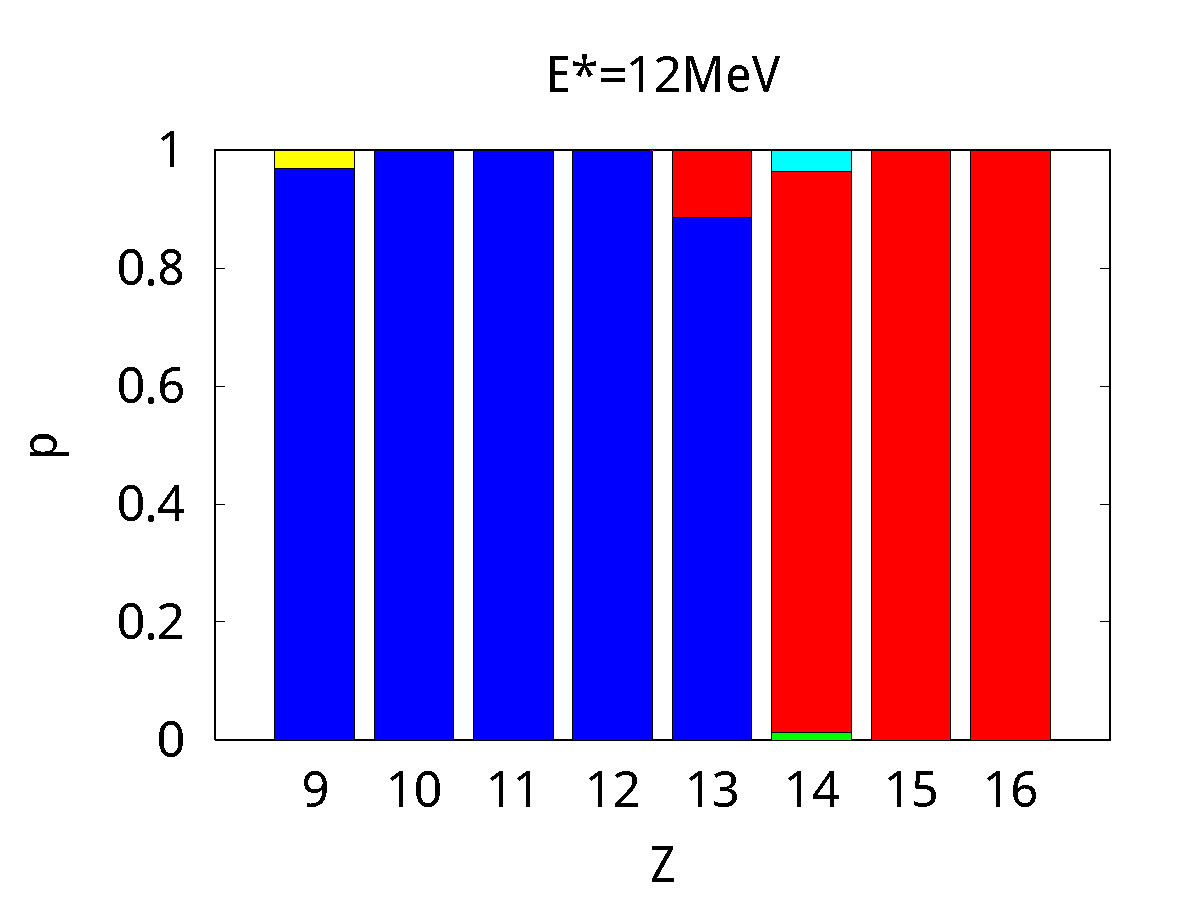
\includegraphics[width=\bredd\textwidth]{figures/bars/12-spectra.pdf}\label{sfig:bars2:12}}
&
\subfloat[$E^{*}=13\,\mathrm{MeV}$]{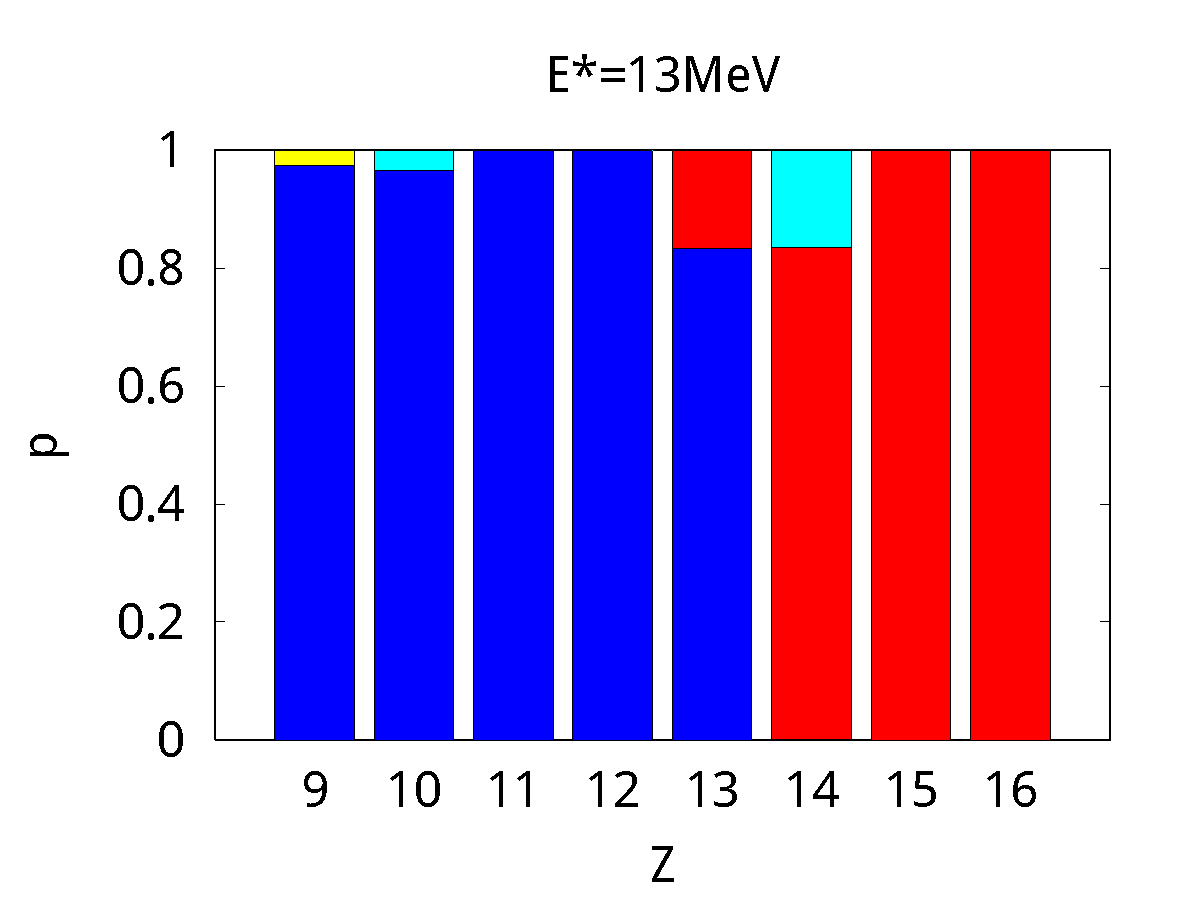
\includegraphics[width=\bredd\textwidth]{figures/bars/13-spectra.pdf}\label{sfig:bars2:13}}
\\
\subfloat[$E^{*}=14\,\mathrm{MeV}$]{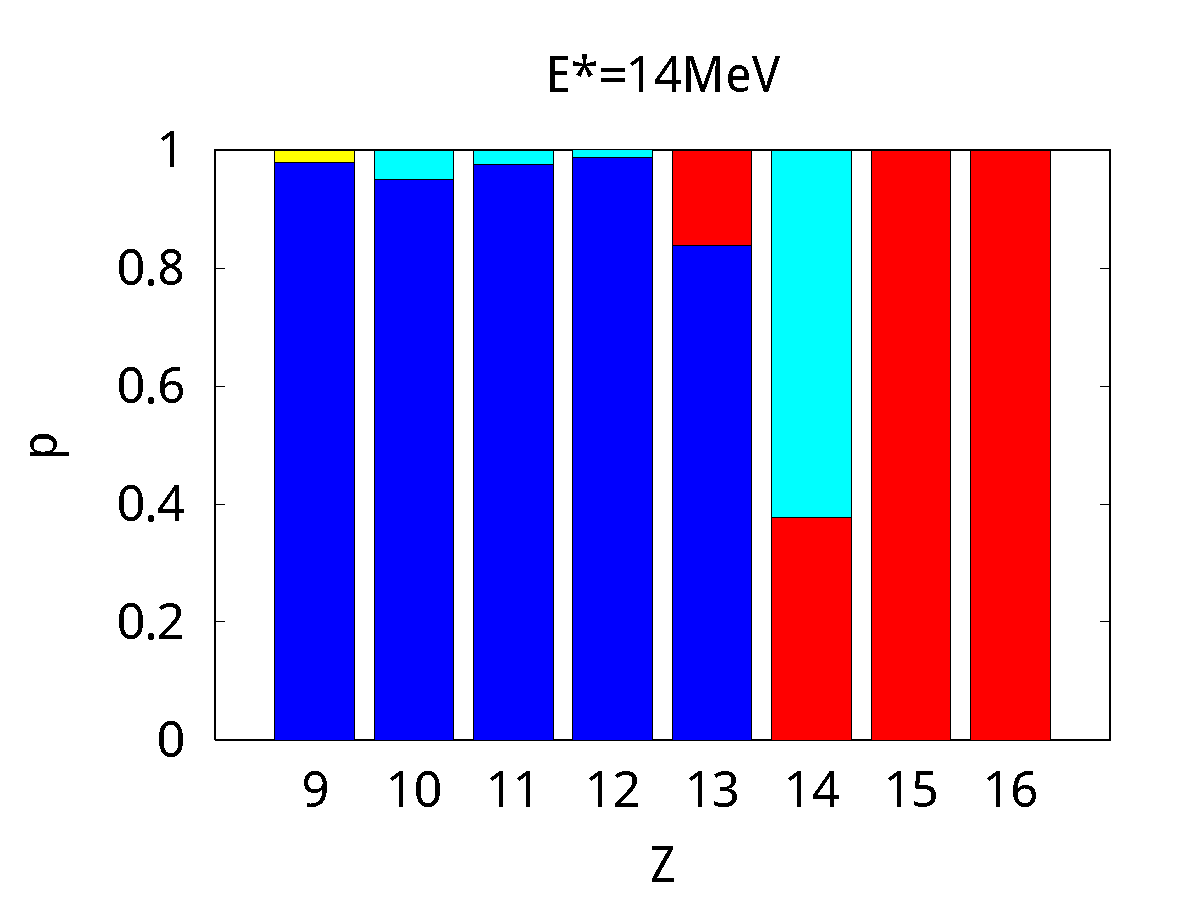
\includegraphics[width=\bredd\textwidth]{figures/bars/14-spectra.pdf}\label{sfig:bars2:14}}
&
\subfloat[$E^{*}=15\,\mathrm{MeV}$]{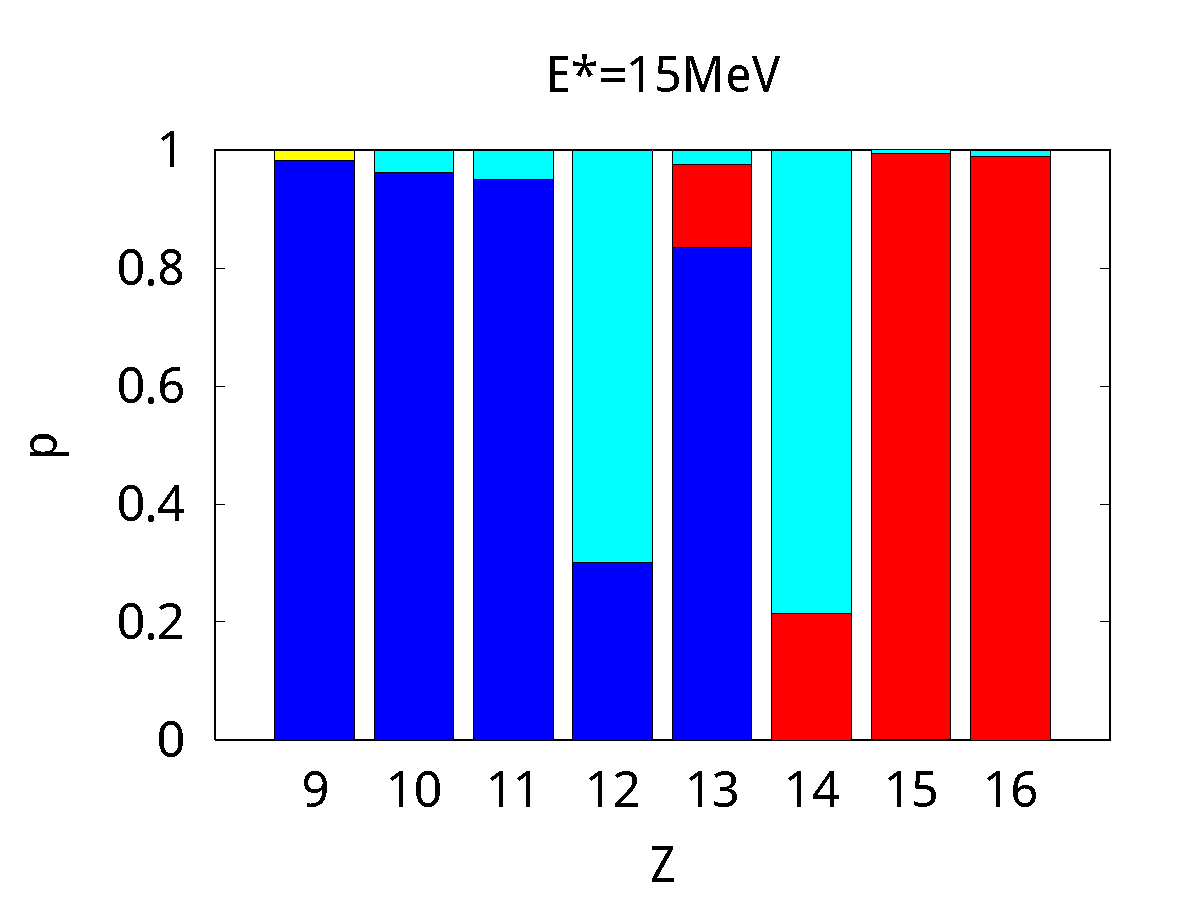
\includegraphics[width=\bredd\textwidth]{figures/bars/15-spectra.pdf}\label{sfig:bars2:15}}
\end{tabular}
\caption{\label{fig:bars2} The branching ratios for various decay modes at various energies for nuclei in the $A=28$, according to \codename{}. The spin is $J=0$ in all cases. The energies have been chosen to display changes in the spectrum. The colors signify the different decay modes: blue=neutron, red=proton, green=gamma, yellow=triton, black=deuteron}
\end{center}
\end{figure}
\endpage{
\begin{figurehere}
\begin{center}
\begin{tabular}{cc}
\subfloat[$E^{*}=16\,\mathrm{MeV}$]{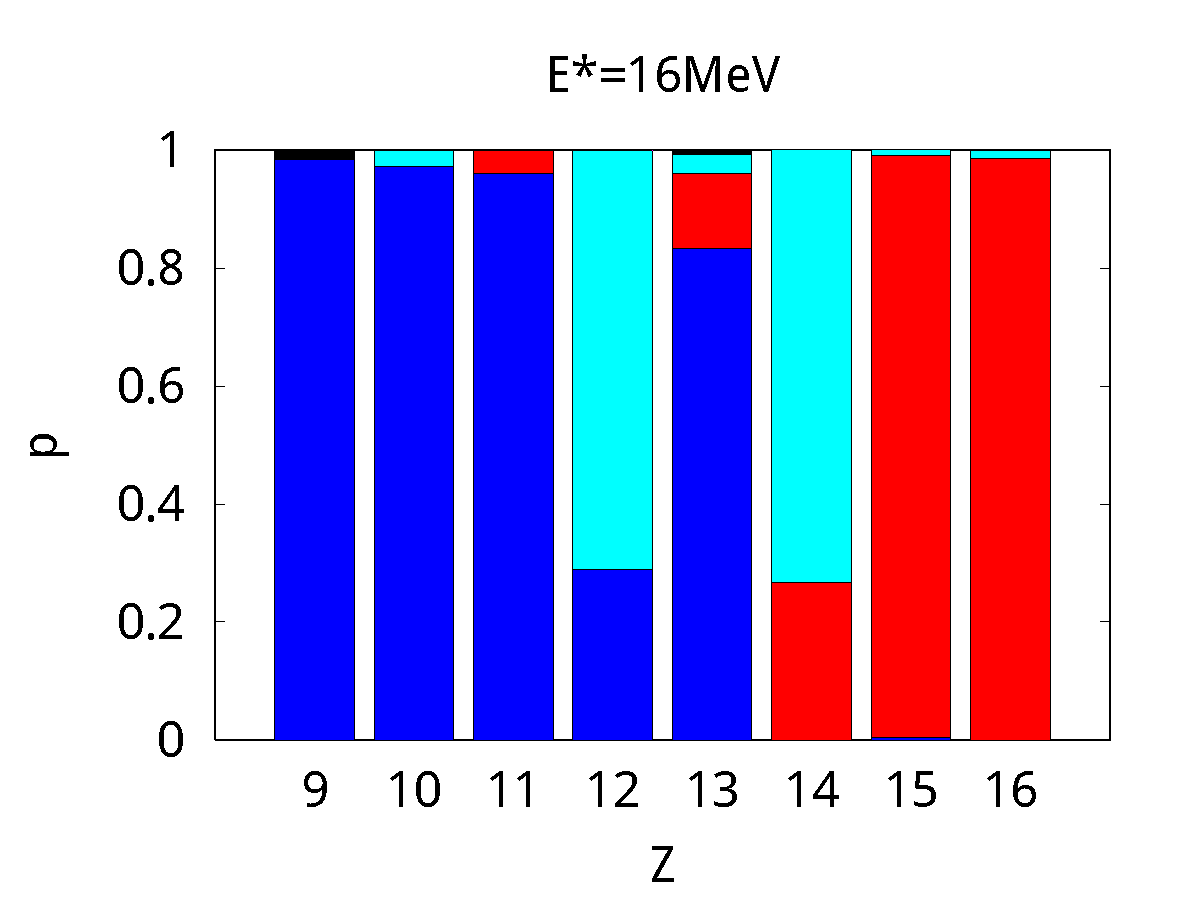
\includegraphics[width=\bredd\textwidth]{figures/bars/16-spectra.pdf}\label{sfig:bars3:16}}
%&
%\subfloat[$E^{*}=18\,\mathrm{MeV}$]{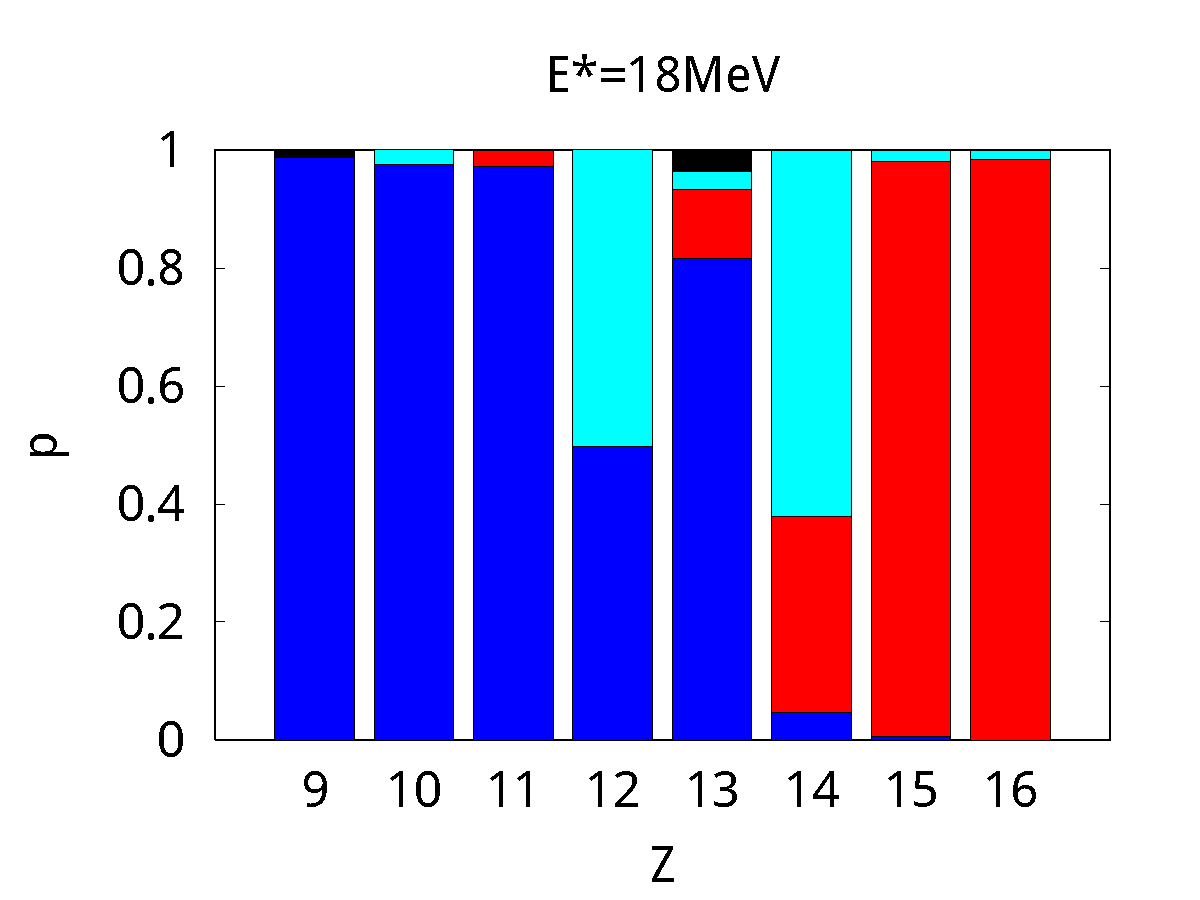
\includegraphics[width=\bredd\textwidth]{figures/bars/18-spectra.pdf}\label{sfig:bars3:18}}
%\\
%\subfloat[$E^{*}=19\,\mathrm{MeV}$]{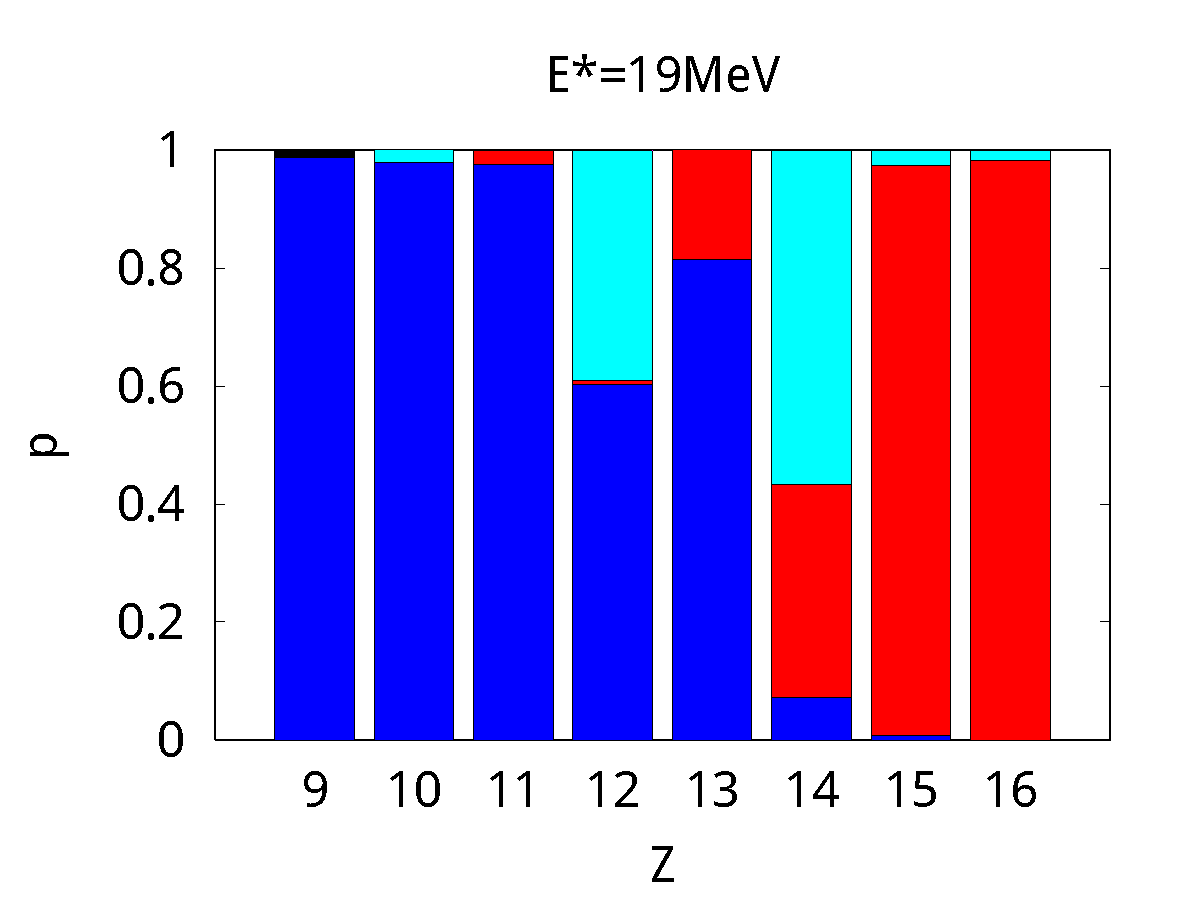
\includegraphics[width=\bredd\textwidth]{figures/bars/19-spectra.pdf}\label{sfig:bars3:19}}
&
\subfloat[$E^{*}=20\,\mathrm{MeV}$]{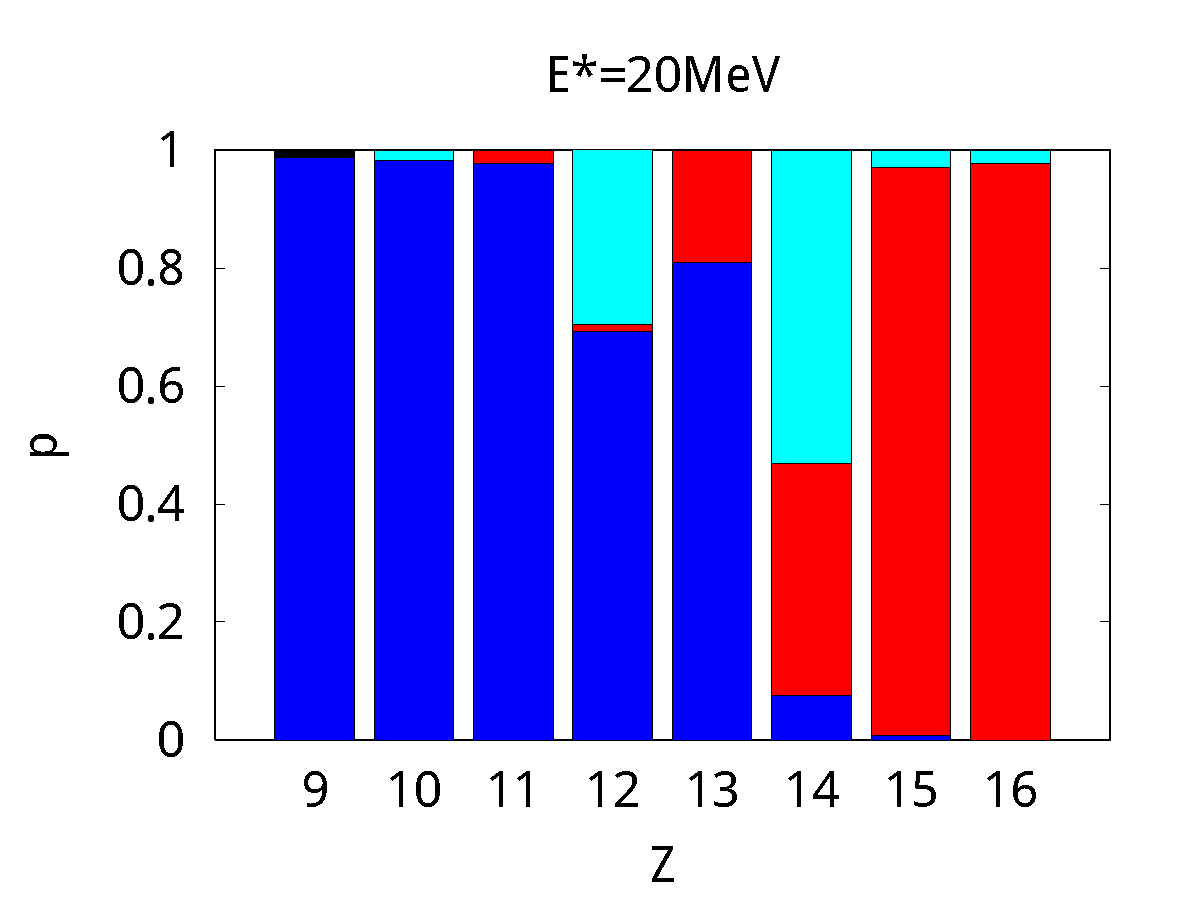
\includegraphics[width=\bredd\textwidth]{figures/bars/20-spectra.pdf}\label{sfig:bars3:20}}
\end{tabular}
\caption{\label{fig:bars3} The branching ratios for various decay modes at various energies for nuclei in the $A=28$, according to \codename{}. The spin is $J=0$ in all cases. The energies have been chosen to display changes in the spectrum. The colors signify the different decay modes: blue=neutron, red=proton, green=gamma, black=deuteron}
\end{center}
\end{figurehere}
\vspace{-5ex}
\begin{figurehere}
\begin{center}
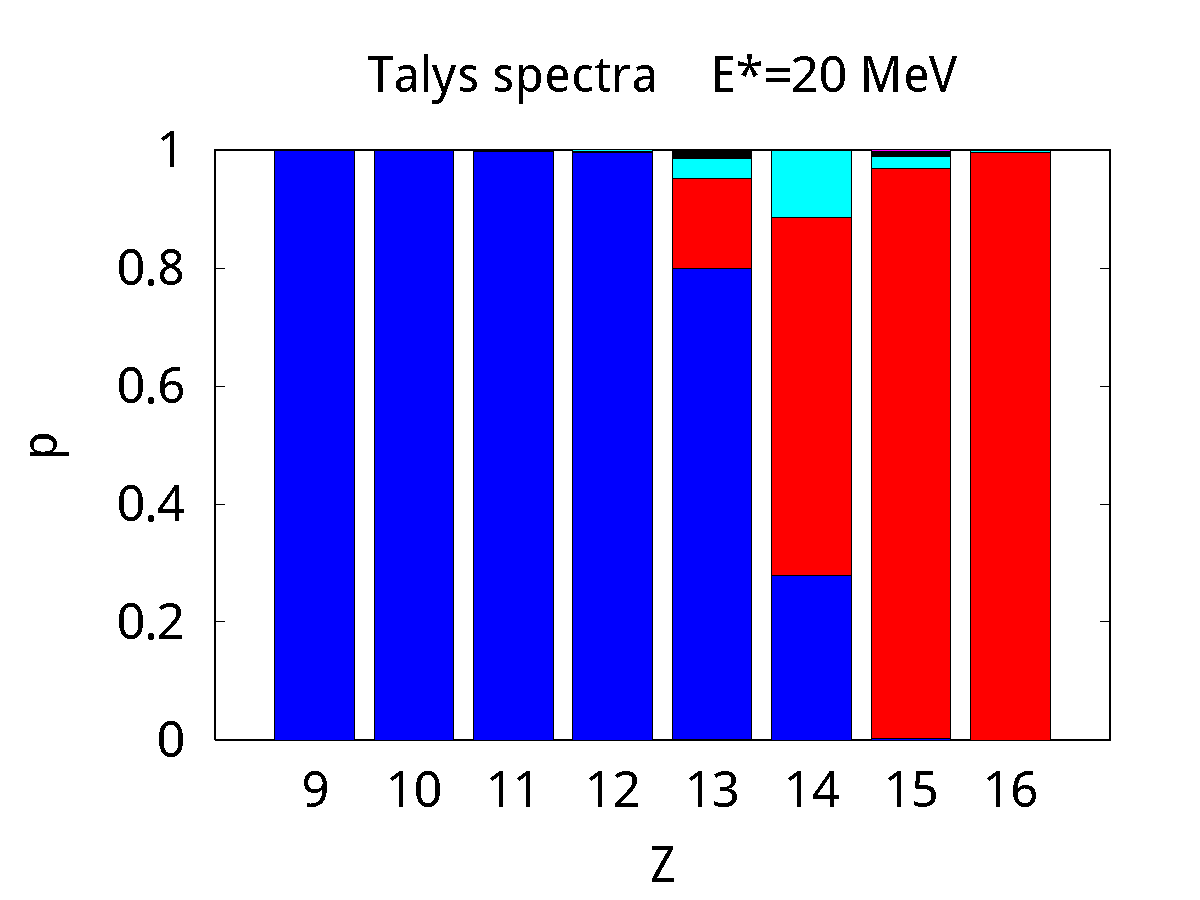
\includegraphics[width=\bredd\textwidth]{figures/bars/20-t-spectra.pdf}
\caption{\label{fig:barst} The branching ratios for various decay modes at $E^*\approx\unit[20]{MeV}$ for nuclei in the $A=28$ isobar, according to \prgname{Talys}. The colors signify the different decay modes: blue=neutron, red=proton, green=gamma, black=deuteron. The spin has been determined by \prgname{Talys}, which populates discrete levels close to $\unit[20]{MeV}$. Plotted is the decay modes from the highest such level.}
\end{center}
\end{figurehere}
}
\clearpage
To investigate how the individual decay modes vary with energy, we finally take a look at the full, energy dependent emission spectrum of a single nucleus.
To see how the $\alpha$-decay mode manages to compete with proton and neutron evaporation, we have plotted the likelihood of $~^{28}\mathrm{Mg}$ emitting protons, alphas and neutrons, for various $l$; see \autoref{fig:fullspec1} and \autoref{fig:fullspec2}. As we see in these figures, which shows the energy cost off emitting the particles\footnote{We plot $E_i^*-E_f^*$ rather than the kinetic energy of the emitted particle, $E_i^*-E_f^*-S$, in order to shift the graphs so that the probabilities become non-zero at $\Delta E = S$, which makes it easier relate the likelihoods of emission to the excitation energy of the mother nucleus. Note however that the relative emission probabilities are unrelated to the excitation energy of the initial state provided that it has enough energy to emit the most likely particle: the $\rho(E_i^*,J_i)$ cancel each other.}, $E_i^*-E_f^*$, each particle has a most likely excitation energy to be emitted at. This is due to the fact that highly excited particles ``saturate'' their transmission coefficients, one $l$ at a time, but because the lowest energy to tunnel through the centrifugal barrier (in our model) goes like $l(l+1)$, the particles are only able to saturate a relatively low number of $T_l$'s until they carry away so much energy that $\rho(E_f^*)$ becomes negligable in comparison to its value at higher $E_f^*$. 
Alpha particles, which have a lower centrifugal barrier, are able to saturate five $l$-values, while protons and neutrons only saturate two, which is reasonably given that $4(4+1)/(2(2+1)) = \frac{10}{3} \approx 4$, which is the ratio relating the nucleon and alpha centrifugal barrier. 
We also see that each $l$ for neutron and proton emission has two curves, related to the fact that there are two ways to couple the spin of the nucleons (the initial state has $J=0$). The alpha particle, being a spin zero particle, only has one curve for each $l$.

In short: a particle carrying away a lot of energy will easily tunnel, but the level density of the final state is much, much higher if the particle carries away just a small amount of energy, and thus high energy emission is effectively supressed, and we get a peak in the emission probabilities for the respective particles. Once our excitation energy is above these peaks, they may be emitted by the most likely way, and hence that probability gets saturated. That being said, the branching ratios can of course benefit from less likely ways to emit, and excitation energies beyond the peak makes the tail of the distribution available for the decays, but we do not expect to see dramatic swings like in the alpha spectrum for $~^{28}\mathrm{Mg}$ between $\unit[14]{MeV}$ and $\unit[15]{MeV}$ in \autoref{fig:bars2}, which coincides rather nicely with the peak in \autoref{sfig:fulla}.

\begin{figure}
\begin{center}
\caption{\label{fig:fullspec1} The simulated probability that $~^{28}\mathrm{Mg}$ decays by proton emission (\ref{sfig:fullp}) and neutron emission (\ref{sfig:full1n}), respectively.}
\begin{tabular}{c}
\subfloat{\scalebox{0.7}{\input{figures/fullspec/Mg28-p.pdf_t}\label{sfig:fullp}}}
\\
\subfloat{\scalebox{0.7}{\input{figures/fullspec/Mg28-n.pdf_t}\label{sfig:full1n}}}
\end{tabular}
\end{center}
\end{figure}

\begin{figure}
\begin{center}
\caption{\label{fig:fullspec2} The simulated probability that $~^{28}\mathrm{Mg}$ decays by alpha emission.}
\begin{tabular}{c}
{\scalebox{0.7}{\input{figures/fullspec/Mg28-a.pdf_t}\label{sfig:fulla}}}
\end{tabular}
\end{center}
\end{figure}

